\documentclass[12pt]{report}
\usepackage[a4paper, total={16cm, 24cm}]{geometry}
\usepackage[greek]{babel}	
\usepackage[Glenn]{fncychap}
\usepackage[version=4]{mhchem}
\usepackage[backend=biber, sorting=none]{biblatex}
\usepackage{listings}
\usepackage{multicol}
\usepackage{xcolor}
\usepackage{caption}
\usepackage{subcaption}
\usepackage{graphicx}
\usepackage{wrapfig}
\usepackage{gfsdidot}
\usepackage{sidecap}
\usepackage{enumitem}
\usepackage{pgfornament}
\usepackage{multirow}
\usepackage{url}

\addbibresource{thesis.bib}
\graphicspath{{img/}}

\definecolor{codegray}{rgb}{0.5,0.5,0.5}
\definecolor{backcolour}{rgb}{0.95, 0.95, 0.92}

\lstdefinestyle{style}{
    backgroundcolor=\color{backcolour},   
    basicstyle=\ttfamily\footnotesize,
    breakatwhitespace=false,         
    breaklines=true,                 
		extendedchars=false,
%		frame=leftline,
    inputencoding=utf8,
    keepspaces=true,                 
		language=Python,
		numbers=left,
    showspaces=false,                
    showstringspaces=false,
    showtabs=false,                  
    tabsize=2
}
\lstset{style=style}

\author{Βεϊσάκης Μανούσος}
\title{Μοντελοποίηση συστημάτων αποθήκευσης, \\με σκοπό την αυξημένη διείσδυση των ΑΠΕ \\στο δίκτυο ηλεκτρικής ενέργειας}
\date{\today}

\begin{document}
\maketitle
\tableofcontents
\chapter*{Ευχαριστίες}
\chapter*{{\latintext{Abstract}}}
Η μεταστροφή σε φιλικότερες για το περιβάλλον πηγές ενέργειας είναι αναπόφευκτη, καθώς η ανάγκη για ένα οικολογικότερο μέλλον, αλλά και η επιβάρυνση των χωρών με τέλη εκπομπών, καθιστούν τις συμβατικές μονάδες παραγωγής ενέργειας
ασύμφορες. Η μεγαλύτερη διείσδυση των ΑΠΕ όμως, στο δίκτυο ηλεκτρικής ενέργειας, προϋποθέτει την ύπαρξη αποθηκευτικών μέσων που θα δεσμεύουν την παραπανήσια ενέργεια που παράγουν οι ΑΠΕ, κατά τις ώρες χαμηλής ζήτησης και θα την 
διαθέτουν στους καταναλωτές, κατά τις ώρες όπου αυτή είναι υψηλότερη. Από τη στιγμή που η παραγωγή των ΑΠΕ εξαρτάται από τις καιρικές συνθήκες, είναι απρόβλεπτη, συνεπώς ένα δίκτυο ηλεκτρικής ενέργειας δεν μπορεί να βασίζεται 
εξ ολοκλήρου σε αυτές.

Σε πολλά μέρη μάλιστα η εγκατάσταση ΑΠΕ φτάνει σε ένα τέλμα, διότι υπερβαίνεται το όριο ισχύς του δικτύου, αλλά και διότι η παραπάνω εγκατάσταση ΑΠΕ, δεν θα προσφέρει περαιτέρω πλεονεκτήματα. Χωρίς κάποιον τρόπο να αποθηκεύεται
η ενέργεια για τις ώρες μεγάλου φόρτου, η παραγώμενη ενέργεια κατά τις ώρες χαμηλής ζήτησης, απλά δεν είναι αξιοποιήσιμη. Επιπλέον, με την αναμενώμενη εξέλιξη του δικτύου σε {\latintext{smart-grid}} και την ένταξη των 
{\latintext{micro-grid}} στην κοινωνία, προβλέπεται να υπάρξουν σημαντικές αλλαγές στον τρόπο που χειριζόμαστε την ενέργεια. Τα έξυπνα δίκτυα εκπροσωπούν μία αμφίδρομη σχέση μεταξύ της παραγωγής και της κατανάλωσης, καθώς ο ίδιος ο 
πολίτης στην σημερινή εποχή, μέσω των ΑΠΕ, μπορεί να είναι παραγωγός. Για τους παραπάνω λόγους η συζητήσεις περί ένταξης μεγάλων σταθμών αποθήκευσης ενέργειας στο δίκτυο, έχουν ενταθεί. 

Στην παρούσα εργασία αναπτύχθηκε ένα πρόγραμμα σε γλώσσα {\latintext{Python}}, το οποίο υπολογίζει το μέγεθος του αποθηκευτικού συστήματος που χρειάζεται μια περιοχή, ώστε οι ΑΠΕ που πρόκειται να προστεθούν στο δίκτυό της να είναι
πλήρως αξιοποιήσιμες. Στα αποτελέσματα του προγράμματος αναγράφεται το κόστος του τελικού συστήματος, καθώς και το πώς θα μεταβληθεί η καμπύλη του φορτίου του δικτύου, μέσω αυτής της προσαρμογής.
\chapter*{Εισαγωγή}
Τον 20ο αιώνα έγινε αντιληπτό ότι ο νέος τρόπος παραγωγής ενέργειας που έφερε η βιομηχανική επανάσταση δεν ήταν βιώσιμος. Πρώτη φορά η ανθρωπότητα είχε την ικανότητα να επηρεάσει σε τέτοιο βαθμό το οικοσύστημα της Γης. Ήταν εμφανές 
πια, ότι έπρεπε να βρεθεί ένας πιο οικολογικός τρόπος για να καλυφθούν οι όλο και αυξανόμενες ανάγκες των ανθρώπων, εάν ήθελε η ανθρωπότητα να αφήσει έναν, αν όχι καλύτερο, έναν ιδίου επιπέδου κόσμο, στις επόμενες γενιές. Έτσι πολλές
χώρες αποφάσισαν να καθιερώσουν νομοθεσίες, οι οποίες θα επιβάλλουν όλο και χαμηλότερη εκπομπή ρύπων διοξειδίου του άνθρακα ({\latintext{\ce{CO2}}}) απ'όλους τους τομείς, προωθώντας μία μεταστροφή σε καθαρότερες πηγές ενέργειας, σε 
αντίθεση με τις συμβατικές μονάδες παραγωγής ηλεκτρικής ενέργειας. Όλο αυτό παρότρυνε τον επιστημονικό και τεχνολογικό τομέα να ερευνήσει ακόμα περισσότερο τις φιλικότερες για το περιβάλλον ενεργειακές πηγές, τις επονομαζόμενες 
Ανανεώσιμες Πηγές Ενέργειας (ΑΠΕ). Λόγω της εξέλιξης της τεχνολογίας, της εύρεσης φθηνότερων υλικών και της μαζικής παραγωγής, οι βιομηχανίες κατάφεραν να μειώσουν το κόστος των ΑΠΕ και παράλληλα να αυξήσουν την αποδοτικότητά τους.
Έτσι οι ΑΠΕ δεν ήταν πια μία ερευνητική ιδέα, αλλά μία πρωσιτή λύση, που συνυπολογίζοντας τα πρόστιμα στα ορυκτά καύσιμα, ανταγωνίζεται τις συμβατικές. Από τα παραπάνω συμπεραίνει κανείς, ότι η μεταστροφή στις ΑΠΕ είναι μονόδρομος και
η μετάβαση αυτή του ενεργειακού τομέα, θα είναι το επίκεντρο των προσοχής για πολλά χρόνια ακόμη.

Παρ'όλα αυτά οι ΑΠΕ έχουν ένα πολύ σοβαρό μειονέκτημα, αυτό της αβεβαιότητας. Σε αντίθεση με τις συμβατικές πηγές ενέργειας (π.χ. λιγνίτης, φυσικό αέριο κ.α.), οι οποίες παρέχουν μία σταθερή παραγωγή, η παραγωγή των ΑΠΕ βασίζεται, 
εκ φύσεως, στις καιρικές συνθήκες. Αυτό παρουσιάζει πολλές δυσκολίες όσον αφορά την ένταξή τους στο δίκτυο ηλεκτρικής ενέργειας. Αρχικά δεν μπορεί ένα κράτος να βασιστεί σε αυτές για την πλήρη κάλυψη του φορτίου του, χωρίς να υπάρχει
σε ένα βαθμό μία σταθερή πηγή ενέργειας, πάνω στην οποία θα ενταχθούν οι ΑΠΕ. Για παράδειγμα, τα φωτοβολταϊκά (ΦΒ) παράγουν ισχύ μόνο τις ώρες με συγκεκριμένη ηλιοφάνεια, ενώ το μεγαλύτερο φορτίο στο δίκτυο παρουσιάζεται τις
απογευματινές ώρες. Αυτό σημαίνει ότι ενώ μπορεί να υπάρχει επαρκή ισχύς ΑΠΕ σύμφωνα με τις ανάγκες του δικτύου, αυτή δεν παράγεται τις αναγκαίες ώρες, με συνέπεια όλη αυτή η παραγώμενη ενέργεια, να μην είναι αξιοποιήσιμη. Οι ΑΠΕ 
δηλαδή εξυπηρετούν μέχρι στιγμής, την κάλυψη του φορτίου αιχμής ενός δικτύου (ξαφνικές διακυμάνσεις πάνω από το σύνηθες) και η διείσδυσή τους πάνω από ένα βαθμό, έχει περισσότερα κόστη, παρά οφέλη. 

Ο μόνος τρόπος για να είναι εφικτή η άυξηση της διείσδυσης των ΑΠΕ στο δίκτυο και ίσως η εξ ολοκλήρου τροφοδοσία του δικτύου με αυτές, είναι να υπάρχει τρόπος να αποθηκευτεί η παραπανήσια ενέργεια κατά την ώρα παραγωγής της και η 
διάθεσή της στο δίκτυο κατά τις ώρες αυξημένης ζήτησης. Ευτυχώς, η αποθηκευτική τεχνολογία έχει αναπτυχθεί σε μεγάλο βαθμό τις τελευταίες δεκαετίες (βλ. Κεφάλαιο \ref{chap:storage}), που δίνεται η δυνατότητα επιλογής διαφορετικών 
αποθηκευτικών μέσων, ανάλογα με τις ανάγκες. Κάποια απευθήνονται για παράδειγμα σε μακρυπρόθεσμες αποθηκεύσεις, ενώ άλλα μπορεί να απευθύνονται σε ανάγκες υψηλής ισχύος. 

Η ένταξη των ΑΠΕ και πόσο μάλλον των αποθηκευτικών συστημάτων στο δίκτυο, θα πρέπει να συνοδευτεί με μεταρρυθμίσεις στην ίδια τη λειτουργία του δικτύου. Μέχρι σήμερα, το δίκτυο ηλεκτρικής ενέργειας ακολουθεί το συμβατικό σχήμα 
παραγωγού-καταναλωτή. Όταν είχε πρωτοσχεδιαστεί αυτή η διάταξη δεν είχε υπολογιστεί, ότι και ο ίδιος ο καταναλωτής θα μπορεί να γίνει παραγωγός και να προσφέρει ενέργεια στο δίκτυο. Στη σημερινή εποχή όμως, η εγκατάσταση ΑΠΕ σε 
οικιακό επίπεδο είναι κάτι το όλο και πιο σύνηθες; η σχέση μεταξύ παραγωγού και καταναλωτή γίνεται αμφίδρομη. Αυτή την ανάγκη έρχονται να εξυπηρετήσουν τα έξυπνα δίκτυα ({\latintext{smart-grids}}). Σε συνδυασμό με τα ηλεκτρικά 
αυτοκίνητα\footnote{Την στιγμή που γράφεται το κείμενο κατατίθεται νομοσχέδιο προς ψήφιση στην ελληνική Βουλή, για την απαγόρευση πώλησης αυτοκινήτων εσωτερικής καύσης από το 2035, αλλά και υποχρεωτικής χρήσης αυτοκινήτων μηδενικών 
εκπομπών για τα ταξί εντός Αττικής και Θεσσαλονίκης από το 2027.}, οι μπαταρίες αυτές θα μπορούν να τροφοδοτούν το δίκτυο με επιπρόσθετη ενέργεια σε συνθήκες υψηλής ζήτησης.

\begin{wrapfigure}{r}{0.4\textwidth}
				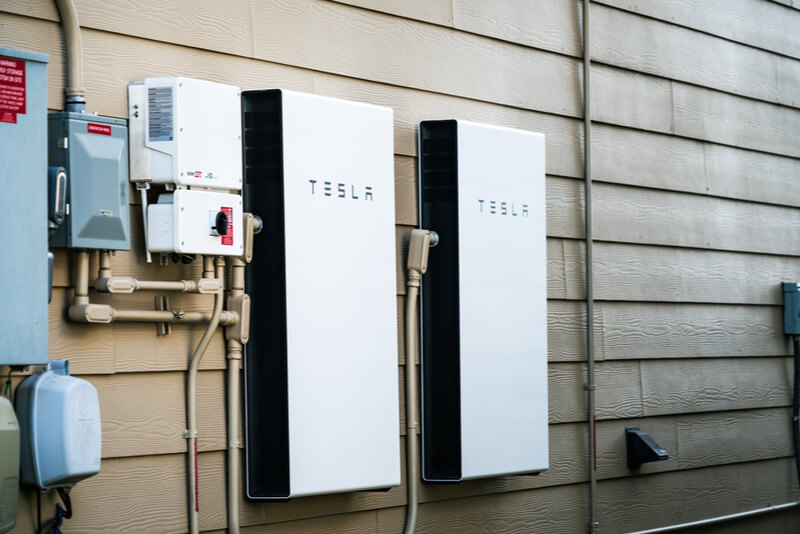
\includegraphics[width=0.4\textwidth]{powerwall}
				\captionsetup{name=Εικόνα}
				\caption{{\latintext{Tesla Powerwall}}.}
				\label{fig:powerwall}
\end{wrapfigure}

Αντίστοιχη χρήση έχει αρχίσει και σε πειραματικό επίπεδο στο εξωτερικό με τις οικιακές μπαταρίες (βλ. Εικόνα \ref{fig:powerwall}). Αυτές αρχικά μπορούν να χρησιμοποιηθούν για ασφάλεια σε περιοχές με συχνές διακοπές ρεύματος, με το 
να αποθηκεύουν ηλεκτρική ενέργεια από το δίκτυο και να τροφοδοτούν το σπίτι σε περίπτωση διακοπής. Υπάρχει η λειτουργία μάλιστα να προγραμματιστεί η μπαταρία να απορροφάει ενέργεια από το δίκτυο μόνο τις ώρες με φθηνότερο κόστος 
(π.χ. νυχτερινό ρεύμα). Η πραγματική αξία όμως αυτών των τεχνολογιών εμφανίζεται όταν συνδυαστούν με ΑΠΕ. 

Όση παραγωγή ενέργειας δεν αξιοποιείται επιτόπου, αποθηκεύεται στις μπαταρίες, από τις οποίες ο χρήστης αντλεί ενέργεια για τις βραδυνές τους καταναλώσεις. Με την χρήση των έξυπνων δικτύων που προαναφέρθηκαν, ο παραγωγός και ο 
καταναλωτής μπορούν να έχουν αμοιβαίο κέρδος. Το δίκτυο κάνει ανοιχτή πρόσκληση σε όποιον ενδιαφερόμενο, ώστε να μπορεί να του αντλεί ενέργεια από τις μπαταρίες του, συγκεκριμένες περιόδους του χρόνου (π.χ. Ιούλιος-Σεπτέμβριος που 
υπάρχει η μέγιστη ζήτηση). Κάθε περισταστικό διαρκεί κάποιες ώρες (συνήθως τις μεσημεριανές), ενώ υπάρχει όριο στα πόσα περιστατικά θα μπορεί να υπάρξουν στον ενδιαφερόμενο μέσα σε αυτήν την περίοδο (π.χ. 50). Στη συνέχεια το δίκτυο 
είναι υπεύθυνο να πληρώσει το ποσό που έχει εγγυηθεί, το οποίο είναι αρκετά ικανοποιητικό. Με αυτό το ποσό όμως κερδίζουν και οι δύο πλευρές. Το κόστος που θα είχε να λειτουργήσει μία παραπάνω μονάδα παραγωγής ηλεκρικής ενέργειας, 
μόνο για αυτά τα συγκεκριμένα περιστατικά μέσα στην περίοδο, είναι κατά πολύ μεγαλύτερο από την "αγορά" της ενέργειας αυτής από τους ίδιους τους καταναλωτές. Από την άλλη ο καταναλωτής μπορεί να ορίσει το ποσό της ενέργειας που θα 
επιτρέπει να δίνει η μπαταρία στο δίκτυο και αν συνδυαστεί αυτό με κάποιο διάστημα που αυτός λείπει από το σπίτι, τότε η ενέργεια που παράγεται από τις ΑΠΕ στο σπίτι του δεν θα πηγαίνει χαμένη καθώς θα μπορεί να πωλείται ενώ λείπει. 
Με αυτόν τον τρόπο, αν πολλοί κάτοικοι μιας περιοχής ενταχθούν σε αυτό το πρόγραμμα, φτιάχνεται μία μεγάλη εικονική μπαταρία, που στηρίζει το δίκτυό της.

Με την ίδια λογική και με τη χρήση των {\latintext{micro-grid}} θα μπορούν ολόκληρες περιοχές να τροφοδοτούνται σε μεγάλο βαθμό μεταξύ τους, μειώνοντας και το ρίσκο διακοπής ρεύματος από τυχόν βλάβη στον κεντρικό παραγωγό. Οι κάτοικοι
με ΑΠΕ, γεννήτριες, μπαταρίες κ.α. θα υποστηρίζουν το δίκτυο της περιοχής τους, με το αντίστοιχο οικονομικό κέρδος από το δίκτυο. Έτσι βγαίνουν όλοι κερδισμένοι, ακολουθώντας την λογική που αναφέρθηκε στην προηγούμενη παράγραφο.

Όλα αυτά είναι εξελίξεις, στις οποίες τα έξυπνα δίκτυα μπορούν και θα πρέπει να ανταπεξέλθουν. Η ανθρωπότητα περνάει σε μια εποχή που η χρήση της ενέργειας αλλάζει μορφή, γίνεται αμφίδρομη με στόχο την αποδοτικότητα και την οικολογία.
Και για τους πιο ψυχρούς αναγνώστες που δεν πείθονται για το περιβαλλοντικό σκέλος του προβλήματος, οι ΑΠΕ είναι ικανές να καταστήσουν τις χώρες ανεξάρτητες από τρίτους προμηθευτές ορυκτών καυσίμων, αποφεύγοντας τις διακυμάνσεις της 
αγοράς ενέργειας, αλλά και τους οποιουσδήποτε γεωπολιτικούς εκβιασμούς.
\chapter{Παραγωγή Ενέργειας}
Στη σημερινή εποχή, οι περισσότερες από τις συσκευές που χρησιμοποιούν οι άνθρωποι στην καθημερινότητά τους, χρειάζονται ηλεκτρική ενέργεια για να λειτουργήσουν. Οι μεγαλύτερες ηλεκτρικές συσκευές, όπως θερμοσίφωνας ή μηχανές
επαγωγής, τροφοδοτούνται με εναλλασσόμενη τάση, ενώ οι μικρές ηλεκτρονικές συσκευές σαν τους υπολογιστές, χρειάζονται συνεχή τάση για τη λειτουργία τους. Αυτή η ηλεκτρική ενέργεια προέρχεται από το δίκτυο σε συγκεκριμένη μορφή
{\latintext{(230V/400V@50Hz)}} και είναι ευθύνη των ίδιων των συσκευών να μετασχηματίσουν την μορφή αυτή, ανάλογα με τις ανάγκες τους\footnote{Υπολογίζεται ότι το 40\% της ηλεκτρικής ενέργειας του δικτύου, υπόκειται σε τέτοιου είδους
μετατροπή.}.

Αντιστρόφως, για να μπορεί η παραγωγή των ΑΠΕ να ενταχθεί στο δίκτυο ηλεκτρικής ενέργειας, ώστε να είναι αξιοποιήσιμη από τους καταναλωτές, θα πρέπει η παραγώμενη ηλεκτρική ενέργεια να είναι της προαναφερθείσας μορφής. Για τον σκοπό 
αυτό, χρειάζεται πάλι η μεσολάβηση μετατροπέων ηλεκτρικής ενέργειας (συνήθως {\latintext{inverter}}), οι οποίοι εκπληρώνουν αυτόν τον σκοπό με τη χρήση εξειδικευμένων ηλεκτρονικών διατάξεων, τα επονομαζόμενα ηλεκτρονικά ισχύος. Αυτή 
η μετατροπή είναι απαραίτητη, καθώς παρ'ότι μία μικρή απόκλιση της τάσης από την επιθυμητή τιμή, δεν αποτελεί σημαντικό πρόβλημα, μία παραμόρφωση της συχνότητας του δικτύου πάνω από το 1\% μπορεί να επιφέρει καταστροφικά αποτελέσματα
για τις συσκευές που είναι συνδεδεμένες σε αυτό. 

Με το πέρασμα των χρόνων, οι προτάσεις περί άντλησης ενέργειας από εξεζητημένες εγκαταστάσεις, πολλαπλασιάζονται. Συνεχώς γίνεται αναφορά για μελέτες παραγωγής ενέργειας από παλίρροιες ή και από τη διαφορά θερμοκρασίας των υδάτων, 
αλλά παρ'ότι όλες αυτές οι έρευνες παρουσιάζουν τεράστιο ενδιαφέρον, δεν είναι εφαρμόσιμες (ακόμα τουλάχιστον), καθώς διατρέχονται από πολλά τεχνο-οικονομικά προβλήματα. Ούτως ή άλλως, για να ενταχθεί μία τέτοιου είδους τεχνολογία 
στην καθημερινότητά μας θα πρέπει να διαθέτει κάποια προτερήματα (κυρίως οικονομικά), τα οποία θα την κάνουν ελκυστικότερη από άλλες συμβατικές πηγές ενέργειας. Οι τεχνολογίες που έχουν αποδείξει ότι και είναι οικολογικές, αλλά και 
συμφέρουσες οικονομικά, είναι τα ΦΒ και οι ΑΓ και με αυτές θα ασχοληθεί το παρόν κεφάλαιο. 
\section{Φωτοβολταϊκά}
"{\textit{Το 1839, ο Γάλλος φυσικός {\latintext{Edmund Becquerel}} ανακάλυψε ότι ορισµένα υλικά µπορούσαν να παράγουν σπινθήρες ηλεκτρισµού όταν υποβάλλονταν σε ηλιακή ακτινοβολία. Αυτό το φαινόµενο, γνωστό και ως φωτοηλεκτρικό
φαινόµενο, χρησιµοποιήθηκε σε «πρωτόγονα» ηλιακά κελιά από σελήνιο στα τέλη του 18ου αιώνα. Τη δεκαετία του 1950, επιστήµονες στα {\latintext{Bell Labs}}, αναπροσάρµοσαν την τεχνολογία και, χρησιµοποιώντας ως βάση το
πυρίτιο, κατασκεύασαν ηλιακά κελιά τα οποία µπορούσαν να µετατρέψουν ποσοστό περίπου 4\% της ηλιακής ενέργειας απευθείας σε ηλεκτρική ενέργεια.}}" \parencite{teetkm2011}
\\[10pt]
Το φωτοβολταϊκό φαινόμενο βασίζεται στις φυσικές ιδιότητες των ημιαγωγών, οι οποίοι κατατάσσονται στην ενδιάμεση κατηγορία μεταξύ των αγωγών και των μονωτών. Στην ουσία αυτά τα υλικά, τα οποία κατασκευάζονται κατά κύριο λόγο
από πυρίτιο {\latintext{(Si)}} και γερμάνιο {\latintext{(Ge)}}, επιτρέπουν τη διέλευση του ηλεκτρικού ρεύματος υπό προϋποθέσεις. Όσον αφορά τη δομή του, η μία του πλευρά του ημιαγωγού είναι εμπλουτισμένη με πλεόνασμα ηλεκτρονίων 
{\latintext{(N)}}, ενώ η άλλη πλευρά με έλλειμμα {\latintext{(P)}}. Από το σημείο διεπαφής {\latintext{(P-N junction)}} των δύο πλευρών δεν είναι δυνατή η διέλευση ηλεκτρονίων, τα οποία όμως έχουν την τάση να φτάσουν στην άλλη πλευρά.
Στην περίπτωση του φωτοβολταϊκού (ΦΒ), τα φωτόνια που πέφτουν πάνω στην επιφάνειά του, εκτοπίζουν αντίστοιχο αριθμό ηλεκτρονίων, που όμως για τον προαναφερθείσα λόγο δεν μπορούν να φτάσουν στην άλλη πλευρά. Συνδέοντας ένα εξωτερικό 
κύκλωμα, τα ηλεκτρόνια βρίσκουν δίοδο προς την {\latintext{(P)}} πλευρά του ημιαγωγού. Στο αυτό το εξωτερικό κύκλωμα συνδέεται το φορτίο που χρήζει τροφοδοσίας.

\begin{figure}[h]
				\center
				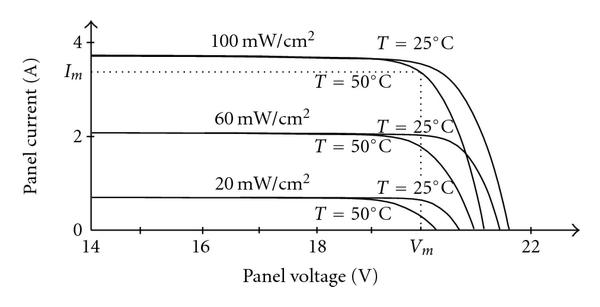
\includegraphics[width=0.8\textwidth]{ivcurve}
				\captionsetup{width=0.9\textwidth}
				\caption{Διαμόρφωση χαρακτηριστικής καμπύλης {\latintext{I-V}} ΦΒ, ανάλογα με τη θερμοκρασία και την ένταση της ηλιακής ακτινοβολίας.}
				\label{fig:ivcurve}
\end{figure}

\begin{wrapfigure}{l}{0.4\textwidth}
				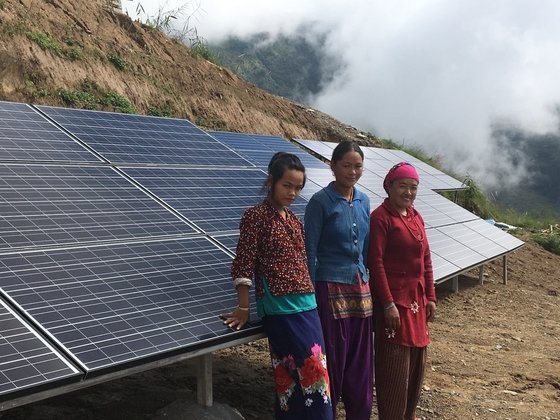
\includegraphics[width=0.4\textwidth]{nepal}
				\captionsetup{name=Εικόνα}
				\caption{Χρήση φωτοβολταϊκών στο Νεπάλ.}
				\label{fig:nepal}
\end{wrapfigure}

Τα φωτοβολταϊκά παρουσιάζουν αρκετές ιδιαιτερότητες στην συμπεριφορά τους, ανάλογα με τις καιρικές συνθήκες, αλλά και τη χρήση τους. Αρχικά αντίθετα απ'ότι θα πίστευε κανείς, τα ΦΒ δεν αρέσκονται στη ζέστη. Ενώ δηλαδή η αυξημένη 
ηλιακή ακτινοβολία, αυξάνει την παραγωγής τους, η ζέστη μειώνει την απόδοσή τους (Σχήμα \ref{fig:ivcurve}). Συγκεκριμένα, ο ρυθμός μεταβολής της τάσης εξόδου του ΦΒ στοιχείου με βάση τη θερμοκρασία περιβάλλοντος είναι περίπου 
-0.3\%/{\latintext{\(^o\)C}}, ενώ το ρεύμα δεν επηρεάζεται σχεδόν καθόλου. Αντίθετα μία αύξηση στην ένταση της ηλιακής ακτινοβολίας επιφέρει αντίστοιχη αύξηση και στο ρεύμα του ΦΒ (γραμμική σχέση), ενώ η αύξηση της τάσης σε αυτήν την 
περίπτωση είναι αμελητέα. Αυτό σημαίνει ότι ιδανικό σενάριο για τις φωτοβολταϊκές εγκαταστάσεις, θα ήταν η κορυφή ενός βουνού με καθαρό ουρανό και πολύ κρύο (Εικόνα \ref{fig:nepal}). Βέβαια αυτό αποτελεί ένα ωραιοποιημένο σενάριο, 
το οποίο εγκυμονεί πολλά πρακτικά προβλήματα. 

Αξίζει να σημειωθεί εδώ, ότι η θερμοκρασία ενός ΦΒ πλαισίου δεν ταυτίζεται πάντα με την θερμοκρασία περιβάλλοντος. Αντίθετα μόνο σε πολύ χαμηλές θερμοκρασίες παρουσιάζεται αυτό, καθώς συνήθως η θερμοκρασία του πάνελ είναι αρκετά 
μεγαλύτερη από τη θερμοκρασία περιβάλλοντος. Ευτυχώς πολλές φορές ο άνεμος στην πίσω πλευρά των πλαισίων λειτουργεί σαν ψυκτικό μέσο, για να δροσίσει και κατά συνέπεια να μειώσει τα ανεπιθύμητα αποτελέσματα των θερμοκρασιακών 
διακυμάνσεων. Είναι σημαντικό επίσης να τονιστεί, ότι η παραγωγή των ΦΒ μειώνεται σε μεγάλο βαθμό σε περίπτωση σκίασης. Το ιδιαίτερο όμως είναι ότι ανάλογα με την φορά της σκίασης, η πτώση στην παραγωγή αλλάζει. Μία σκίαση κατά μία 
συγκεκριμένη διεύθυνση, μπορεί να επιφέρει μεγαλύτερη μείωση στην παραγωγή του πάνελ, απ'ότι μία σκίαση ίδιου μεγέθους, αλλά με άλλη κατεύθυνση. Όλα αυτά θα πρέπει να τα έχει υπόψιν του ο μελετητής, διότι είναι παράγοντες που μπορούν
να επιφέρουν απροσδόκητα αποτελέσματα στο σύστημα. 

Καθώς η συμπεριφορα των ΦΒ διαφοροποιείται σε μεγάλο βαθμό ανάλογα με τις καιρικές συνθήκες, οι κατασκευαστές των ΦΒ αναγράφουν τα τεχνικά χαρακτηριστικά των πλαισίων για συγκεκριμένες περιβαλλοντικές συνθήκες. Οι πιο διάσημες
από αυτές είναι οι {\latintext{Standard Test Conditions (STC)}}, οι οποίες αντιστοιχούν σε θερμοκρασία \textbf{πλαισίου} {\latintext{\ce{25^oC}}}, τιμή μάζας αέρα (ΑΜ) ίση με 1.5 και πυκνότητα ισχύος ηλιακής ακτινοβολίας 
{\latintext{1 kW/\ce{m^2}}}. Βέβαια συμπεραίνει κανείς ότι αυτές οι συνθήκες, είναι το λιγότερο αισιόδοξες. Για τον λόγο αυτό αναπτύχθηκε και ένα άλλο σύστημα συνθηκών το επονομαζόμενο 
{\latintext{Nominal Operating Cell Temperature (NOCT)}}, το οποίο αναφέρεται σε θερμοκρασία \textbf{αέρα} {\latintext{\ce{20^oC}}}, ένταση ηλιακής ακτινοβολίας στην επιφάνεια του πλαισίου ίση με {\latintext{800 W/\ce{m^2}}} 
και ταχύτητα ανέμου ίση με {\latintext{1 m/s}} με ανοιχτή την πίσω πλευρά του πλαισίου. Το δεύτερο σύστημα προσεγγίζει καλύτερα τις πραγματικές καιρικές συνθήκες, στις οποίες θα χρειαστεί να λειτουργήσει ένα ΦΒ πλαίσιο. 

Υπάρχουν διαφορετικοί τύποι ΦΒ ανάλογα με το υλικό και τον τρόπο που έχουν κατασκευαστεί. Τα πιο σύνηθη είναι τα πλαίσια από πυρίτιο, μονοκρυσταλλικού πυριτίου {\latintext{Mono-Si}}, πολυκρυσταλλικού πυριτίου {\latintext{Poly-Si}}, 
είτε και άμορφου {\latintext{a-Si}}. Η διαφορά τους έγκειται στην απόδοση, αλλά και το κόστος. Τα {\latintext{Mono-Si}} είναι τα πιο αποδοτικά\footnote{Η απόδοση των ΦΒ μεταβάλλεται ανάλογα με το υλικό που χρησιμοποιείται, την
κατασκευαστική γεωμετρία, την κρυσταλλική ποιότητα και καθαρότητα, τη θερμοκρασία λειτουργίας και τέλος από τη χροιά και την πυκνότητα της προσπίπτουσας ακτινοβολίας. Για τα {\latintext{Mono-Si}}
ΦΒ η απόδοση μπορεί να ξεπεράσει και τα 20\%, για τα {\latintext{Poly-Si}} η απόδοση είναι γύρω στα 16\%, ενώ για τα {\latintext{a-Si}} η απόδοση είναι πολύ χαμηλή γύρω στα 7\%.}, ενώ τα {\latintext{Poly-Si}} έχουν χαμηλότερο
κόστος και προτιμούνται από τους μέσους χρήστες, χωρίς πολλές απαιτήσεις. Τέλος τα πλαίσια άμορφου πυριτίου χαρακτηρίζονται από χαμηλή απόδοση, αλλά χαμηλό κόστος και βελτιωμένη συμπεριφορά στις συννεφιασμένες καιρικές συνθήκες.

Υπάρχουν και άλλες τεχνολογίες ΦΒ που συμπεριλαμβάνουν άλλα υλικά, όπως γερμάνιο ή κάδμιο, με σκοπό την αυξημένη απόδοση, αλλά το κόστος τους είναι απαγορευτικό και απευθήνονται μόνο σε επιστημονικές μελέτες και διαστημικές
αποστολές. Από την άλλη αναπτύσσονται υλικά που θα επιτρέπουν την ένταξη των ΦΒ στα σπίτια με έναν πιο διακριτικό τρόπο, όπως διαφανή πλαίσια για τα παράθυρα ή φωτοβολταϊκά σε σχήμα κεραμιδιών. Αυτές οι τεχνολογίες όμως, είναι
ακόμα σε ερευνητικό επίπεδο και δεν έχει υπάρξει μαζική παραγωγή τους.

Το ιδιαίτερο με τα ΦΒ συστήματα είναι ότι αποτελούν μία στατική πηγή ενέργειας, σε αντίθεση με τις περισσότερες ΑΠΕ, οι οποίες περιλαμβάνουν μία περιστρεφόμενη διάταξη, η οποία συνοδευόμενη από μία γεννήτρια, παράγει ηλεκτρική
ισχύς. Έτσι τα φωτοβολταϊκά δεν περιλαμβάνουν κινούμενα μηχανικά μέρη, συνεπώς η συντήρησή τους περιορίζεται, κατά κύριο λόγο, στο τακτικό καθάρισμά τους, ενώ η ηλεκτρική τάση που παράγουν είναι συνεχούς μορφής.

Για την μετατροπή της συνεχούς τάσης σε εναλλασσόμενη, ώστε να διανεμηθεί στο δίκτυο ή έστω να χρησιμοποιηθεί από τις απλές οικιακές συσκευές, χρειάζεται η μεσολάβηση ενός αντιστροφέα. Μέσω εξειδικευμένων διατάξεων ηλεκτρονικών
ισχύος, η {\latintext{DC}} μορφή, μετατρέπεται σε {\latintext{AC}} κατάλληλης συχνότητας και τάσης. 

Στην περίπτωση ενός συστήματος συνδεδεμένου με το δίκτυο ({\latintext{on-grid}}), ένας αντιστροφέας και ένας έξυπνος μετρητής αρκούν για την σωστή λειτουργία της εγκατάστασης. Στην περίπτωση όμως μη-συνδεδεμένου με το δίκτυο
συστήματος ({\latintext{off-grid}}), χρειάζονται επιπλέον μπαταρίες και ρυθμιστές φόρτισης, έτσι ώστε να εξασφαλίζεται η ανεμπόδιστη τροφοδοσία ρεύματος και κατά της νυχτερινές ώρες. Προφανώς τα {\latintext{off-grid}}
συστήματα παρουσιάζουν υψηλότερο κόστος, περισσότερη συντήρηση και πιο σύνθετη μελέτη από μεριάς του μηχανικού. Σε γενικές γραμμές τα {\latintext{on-grid}} συστήματα έχουν ένα κόστος των 1500 {\latintext{€/kWp}}, ενώ τα 
{\latintext{off-grid}} περίπου 4000 {\latintext{€/kWp}}.

Αναλύοντας περισσότερο τα κόστη, σε ένα σύστημα θα πρέπει να συνυπολογιστεί και το πόσο προσβάσιμη είναι μία περιοχή και τι είδους παραπανήσιο εξοπλισμό θα χρειαστεί ο μηχανικός για την εγκατάσταση. 
Αν από την άλλη, η περιοχή είναι περιορισμένης έκτασης, τότε θα ήταν προτιμώτερο να τοποθετηθούν ΦΒ πλαίσια αυξημένης απόδοσης ({\latintext{Mono-Si}}), ανεξαρτήτως κόστους, διότι θα είναι εφικτή, η καλύτερη εκμετάλλευση 
της μικρής επιφάνειας του χώρου. Τέλος δεν
πρέπει να παραλειφθεί ότι για λόγους οικονομίας κλίμακας, το κόστος ενός μικρού ΦΒ πάρκου είναι μεγαλύτερο αναλογικά, σε σχέση με ενός μεγάλου, ενώ επίσης ο μελετητής καλό θα είναι να επιλέξει επώνυμα πλαίσια, 
διότι παρά το αυξημένο κόστος τους, παρέχουν στον χρήστη αυξημένη ασφάλεια, λόγω της αξιοπιστίας τους. 
\section{Ανεμογεννήτριες}
Όπως οι περισσότερες μορφές ενέργειας, έτσι και η αιολική βασίζεται στον ήλιο. Συγκεκριμένα η ηλιακή ακτινοβολία που προσπίπτει στη Γη θερμαίνει την επιφάνεια του εδάφους, η οποία με τη σειρά της μεταφέρει τη θερμότητα αυτή 
στις αέριες μάζες που βρίσκονται πάνω από αυτήν. Η αύξηση της θερμοκρασίας μιας αέριας μάζας επιφέρει μείωση στην πυκνότητά της και την ανοδική της πορεία, ενώ αντίστοιχος ψυχρός αέρας μετακινείται για την πλήρωση των κενών
που δημιουργούνται. Αυτή η συμπεριφορά παρατηρείται και σε μακρο-κλίμακα με τις κινήσεις ψυχρών ανέμων από τις βορειότερες περιοχές της Γης προς τις θερμότερες περιοχές του ισημερινού, αλλά και σε μίκρο-κλίμακα, για παράδειγμα 
σε παραθαλάσσιες περιοχές, όπου η διαφορά θερμοκρασίας του αέρα που βρίσκεται πάνω από τη θάλασσα και αυτού που βρίσκεται πάνω από την άμμο είναι αρκετά μεγάλη. Η διαφορά πίεσης συνεπώς που προκαλείται λόγω της ανομοιόμορφης
θέρμανσης του αέρα προκαλεί την κίνηση του, η οποία κίνηση ονομάζεται άνεμος και περιέχει κινητική ενέργεια που μπορεί να αξιοποιηθεί.

Η ταχύτητα του ανέμου καθορίζεται από τις παραπάνω διαφορές θερμοκρασιών, αλλά και από την τοπολογία της περιοχής. Τα φυσικά εμπόδια που μπορεί να συναντήσει ο άνεμος κατά τη διαδρομή του, όπως λόφοι, κτίρια κ.α. διαταράσσουν την
πορεία του και μειώνουν την ολική του κινητική ενέργεια. Συνεπώς μπορεί να υπάρξει καλύτερη εκμετάλλευση της αέριας δέσμης σε επίπεδες περιοχές, ειδικά σε θαλάσσιες ή σε μεγάλα ύψη, όπου η μορφολογία του εδάφους δεν μπορεί να
επηρεάσει πια την πορεία του ανέμου. Επίσης σε συγκεκριμένα περάσματα του αέρα όπως κορυφογραμμές, οι ροϊκές γραμμές του αέρα είναι πιο πυκνές και γι'αυτό αυτά τα μέρη προτιμώνται για την εκμετάλλευση της αιολικής ενέργειας.
Τέλος την κίνηση των αέριων μαζών επηρεάζει και η ιδιοπεριστροφή της Γης, η οποία τις παρασέρνει με ρυθμό που εξαρτάται από το γεωγραφικό πλάτος της περιοχής.

Ο τρόπος αυτός της εκμετάλλευσης γίνεται μέσω ειδικών διατάξεων που περιστρέφονται καθώς ο άνεμος προσπίπτει πάνω σε αυτές, αντλώντας έτσι ένα μέρος της κινητικής ενέργειας του αέρα. Αυτές οι διατάξεις είναι γνωστές ως
ανεμογεννήτριες (Α/Γ) και εμφανίζονται σε δύο κύριες μορφές, οριζοντίου άξονα και καθέτου άξονα, με πιο διαδεδομένες τις πρώτες. Τα παλαιότερα χρόνια η περιστροφική κίνηση των διατάξεων αυτών χρησιμοποιούταν για την άλεση σιτηρών, 
αλλά σήμερα μετατρέπεται κυρίως σε ηλεκτρική ενέργεια, μέσω γεννητριών.

Το 1919 ο γερμανός φυσικός {\latintext{Albert Betz}} διατύπωσε ότι το μέγιστο ποσοστό που μπορεί να αντλήσει μία ανεμογεννήτρια από τον αέρα είναι το 59\%\footnote{Συγκεκριμένα η τιμή αυτή είναι \(16/27\), δηλαδή 0.593 και 
ονομάζεται συντελεστής {\latintext{Betz}}.} της ολικής κινητικής ενέργειας της αέριας δέσμης. Συνεπώς η απόδοση μιας ΑΓ είναι μικρότερη του 59\% και μάλιστα αυξομειώνεται ανάλογα με την ταχύτητα περιστροφής των πτερυγίων της. 
Αυτό συμβαίνει διότι σε μικρές ταχύτητες περιστροφής ένα μεγάλο μέρος του αέρα δεν προλαβαίνει να αξιοποιηθεί, ενώ οι μεγάλες περιστροφικές ταχύτητες δημιουργούν αναταράξεις που δυσχεραίνουν την ομαλή λειτουργία της πτερωτής.

\begin{figure}[t]
				\center
				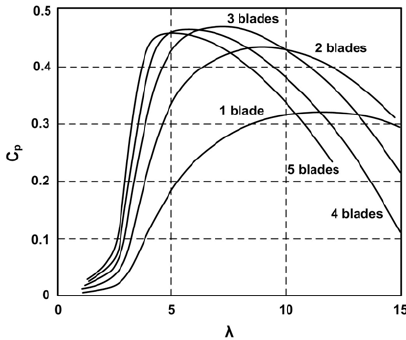
\includegraphics[width=0.8\textwidth]{cp}
				\captionsetup{width=0.9\textwidth}
				\caption{Η απόδοση της ΑΓ συναρτήση του πηλίκου ταχύτητας ακροπτερυγίου λ = {\latintext{\(\omega\cdot\frac{R}{w}\)}}, όπου ω η γωνιακή ταχύτητα του δρομέα της ΑΓ, {\latintext{R}} η ακτίνα του πτερυγίου του και 
								{\latintext{w}} η ταχύτητα του ανέμου. Από το διάγραμμα είναι εμφανής ο λόγος που χρησιμοποιούνται τρία πτερύγια στις ΑΓ, καθώς παραπάνω από αυτόν τον αριθμό επιφέρεται μικρό κέρδος σε σχέση με το αντίστοιχο κόστος.}
				\label{fig:cp}
\end{figure}

Η κίνηση του ανέμου σε αντίθεση με την ηλιακή ακτινοβολία δεν είναι τόσο προβλέψιμη ή τουλάχιστον δεν είναι τόσο περιοδική και επαναλαμβανόμενη. Παρ'όλο που υπάρχουν αρκετά εξεζητημένα προγράμματα που προβλέπουν τις ταχύτητες 
του αέρα, είναι τόσοι πολλοί οι παράγοντες που καθορίζουν την πορεία του ανέμου, που θεωρείται σχεδόν τυχαία. Συνεπώς για την μοντελοποίηση αιολικών συστημάτων χρησιμοποιούνται σε μεγάλο βαθμό στατιστικά μοντέλα και κατανομές
πιθανοτήτων. Η πιο διάσημη κατανομή είναι η κατανομή {\latintext{Weibull}}, η οποία παρουσιάζει το πόσο πιθανό είναι να βρεθεί μία τιμή ταχύτητας του ανέμου σε ένα διάστημα ταχυτήτων.

\begin{table}[h]
\centering
				\begin{tabular}{|c|c|c|c|c|}
				\hline
				\multirow{2}{2.9cm}{Μέγεθος ΑΓ} & \multirow{2}{2.9cm}{Ισχύς Εξόδου ({\latintext{kW}})} & \multirow{2}{2.9cm}{Ύψος Πύργου ({\latintext{m}})} & 
				\multirow{2}{2.9cm}{Διάμετρος Ρότορα ({\latintext{m}})} & \multirow{2}{2.9cm}{Επιφάνεια σάρωσης ({\latintext{m\(^2\)}})} \\[24pt]
				\hline
				{\latintext{micro}} & \(<\)1 & - & \(<\)2.1 & \(<\)3.5 \\
				\hline
				Μικρό & 1-50 & 5-30 & 2.1-16 & 3.5-200 \\
				\hline
				Μεσαίο & 50-1000 & 30-70 & 16-55 & 200-2400 \\
				\hline
				Μεγάλο & \(>\)1000 & \(>\)50 & \(>\)55 & \(>\)2400 \\
				\hline
				\end{tabular}
\captionsetup{width=0.8\textwidth}
\caption{Ταξινόμηση μεγεθών Α/Γ.}
\label{tab:wt-size}
\end{table}

Η κινητική ενέργεια του ανέμου, όπως προαναφέρθηκε, μετατρέπεται σε περιστροφική κίνηση στον άξονα της ΑΓ. Επειδή οι υψηλές στροφές είναι επικίνδυνες για τυχόν ατυχήματα, αλλά προκαλούν επίσης και ηχητικές ενοχλήσεις, η πτερωτή 
περιστρέφεται γύρω στις 20-50 στροφές το λεπτό. Για την παραγωγή ηλεκτρικής τάσης κατάλληλου πλάτους και συχνότητας χρειάζονται όμως περισσότερες στροφές και για τον λόγο χρησιμοποιείται στις ΑΓ κατάλληλο κιβώτιο ταχυτήτων. Με τη
σειρά του αυτό συνδέεται στη γεννήτρια εναλλασσομένου ρεύματος. Για τις περιπτώσεις υψηλών ταχυτήτων ανέμου που μπορεί να προκαλέσουν υπερβολικές ταχύτητες της πτερωτής με καταστρεπτικές συνέπειες, αλλά και για τυχόν συντηρήσεις που
χρειάζονται να λάβουν χώρα, εγκαθίστονται συστήματα πέδησης τα οποία μπορούν να σταματήσουν την περιστροφή της πτερωτής. Με κατάλληλους αισθητήρες διεύθυνσης ανέμου (ανεμοδείκτης) και μέσω ηλεκτρονικών συστημάτων, η ΑΓ έχει τη
δυνατότητα να περιστρέφεται ως προς τον κάθετο άξονά της, ώστε η διεύθυνση του ανέμου να είναι πάντα κάθετη προς την επιφάνεια σάρωσης της πτερωτής. Όλα αυτά τα συστήματα τοποθετούνται στην άτρακτο της ΑΓ και μέσω του κλιμακοστασίου
που βρίσκεται μέσα στον πύργο της, επιτρέπεται η πρόσβαση των μηχανικών στο μηχανοστάσιο αυτό.

Υπάρχουν κυρίως δύο τύποι γεννητριών που παράγουν ηλεκτρική ενέργεια. Ο πρώτος και πιο απλός είναι η περιστροφή της πτερωτής με σταθερή ταχύτητα, με συνέπεια η παραγωγή της ασύγχρονης γεννήτριας που χρησιμοποιείται σε
αυτήν την περίπτωση να είναι σταθερή. Στην διάταξη αυτή λόγω των επαγωγικών στοιχείων εγκαθίστονται κατάλληλου μεγέθους πυκνωτές, ώστε να πλησιάσει ο {\latintext{cos}}φ την μονάδα. Η άλλη περίπτωση περιλαμβάνει την χρήση σύγχρονης
γεννήτριας για συστήματα που η ταχύτητα περιστροφής της πτερωτής δεν είναι σταθερή. Σε αυτήν την περίπτωση η παραγώμενη εναλλασσόμενη τάση μετατρέπεται δύο φορές, αρχικά από {\latintext{AC}} σε {\latintext{DC}} (ανόρθωση) και στη
συνέχεια από {\latintext{DC}} πάλι σε {\latintext{AC}} (αντιστροφή). Με αυτόν τον τρόπο εξασφαλίζεται ότι ανεξάρτητα από την μορφή της αρχικά παραγώμενης τάσης, η τελική μορφή που θα δέχεται το δίκτυο θα πληρεί τις προδιαγραφές. 

Όλα αυτά τα συστήματα χρήζουν τακτικής συντήρησης, ειδικά λόγω των πολλών κινούμενων μερών. Σε αντίθεση με τα ΦΒ που δεν περιέχουν κανένα κινούμενο μέρος (συνεπώς και ελάχιστη συντήρηση), οι ΑΓ περιέχουν περιστρεφόμενα μέρη, κιβώτια
ταχυτήτων και άλλα κινούμενα μέρη, τα οποία χωρίς συντήρηση μπορούν να προκαλέσουν καταστροφικές βλάβες στο σύστημα. Οι υψηλές ταχύτητες του αέρα μάλιστα και οι ρυπές του ανέμου, προκαλούν δονήσεις στην ανεμογεννήτρια που μπορούν να
χαλαρώσουν τις συνδέσεις ή και να καταστρέψουν εντελώς κάποια εξαρτήματα.

\chapter{Αποθήκευση Ενέργειας}
\label{chap:storage}
Η αποθήκευση ενέργειας δεν είναι μία καινούργια ανησυχία. Ανέκαθεν ο άνθρωπος αναζητούσε τρόπους να δεσμεύσει ενέργεια για μελλοντική χρήση, απλά τώρα υπάρχει η κατάλληλη τεχνολογία. 
Με την μεταστροφή σε ένα πιο πράσινο μέλλον έχουν αναπτυχθεί πολλές διαφορετικές τεχνολογίες που εξυπηρετούν ξεχωριστούς σκοπούς, όσον αφορά την αποθήκευση. Οι κύριες τεχνολογίες και οι χρήσεις τους που απασχολούν
τον επιστημονικό τομέα
είναι οι μπαταρίες (κυρίως Λιθίου-Ιόντος) για τα φορτία αιχμής του δικτύου και το υδρογόνο για μακροβιότερες αποθηκεύσεις. Παρ'όλα αυτά δεν θα πρέπει να λησμονείτε η αξιόπιστη αντλησιοταμίευση από αυτές τις τεχνολογίες. 
Στο κεφάλαιο αυτό θα αναφερθούν συνοπτικά αυτές οι κύριες τεχνολογίες αποθήκευσης που απασχολούν τον ενεργειακό τομέα, των οποίων η χρήση δεν είναι απλά επιστημονικά ενδιαφέρουσα, αλλά και οικονομικά συμφέρουσα.

\begin{figure}[h]
				\center
				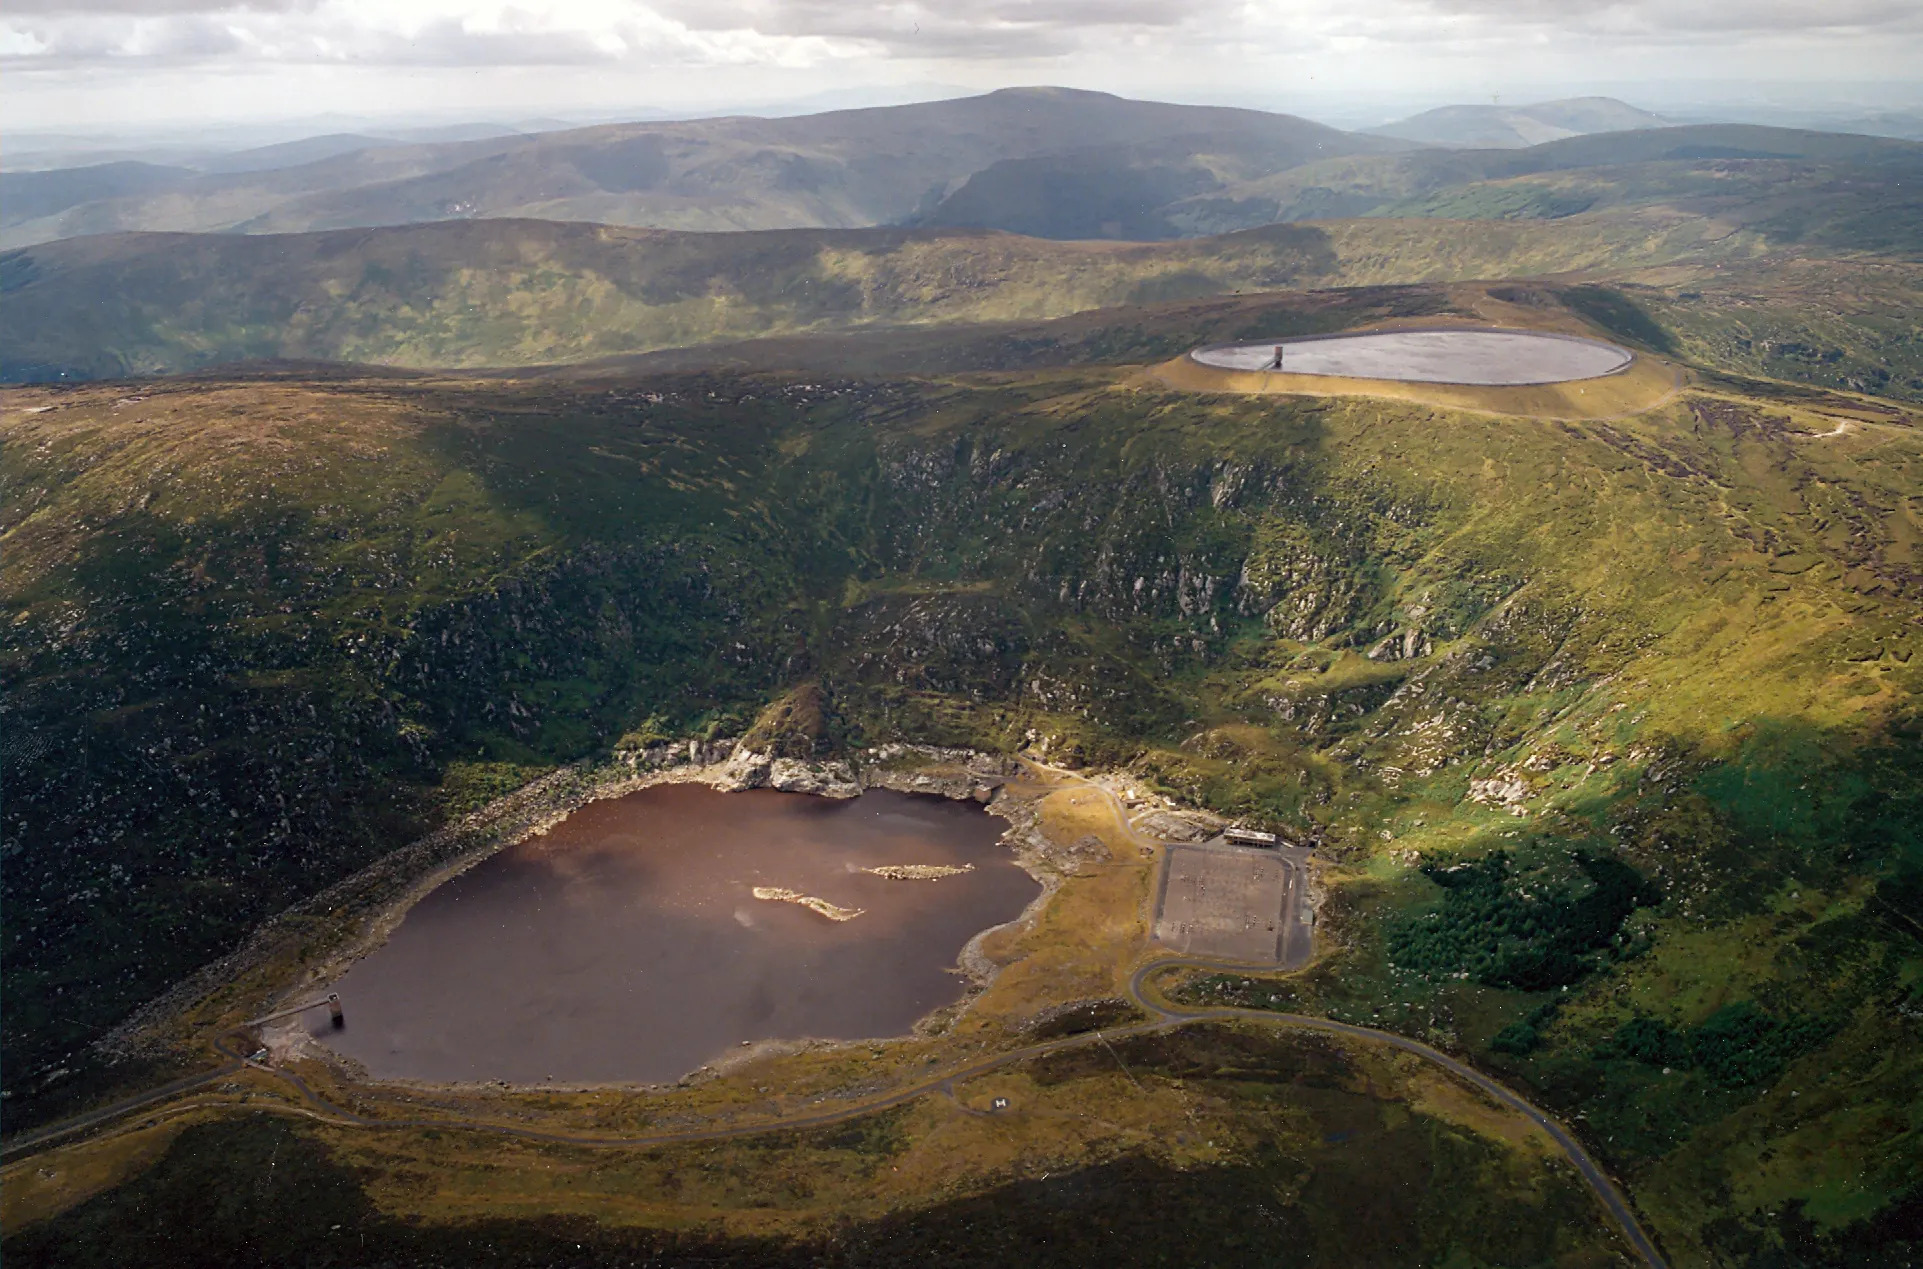
\includegraphics[width=0.7\textwidth]{turlough-hill}
				\captionsetup{name=Εικόνα, width=0.8\textwidth}
				\caption{Το μοναδικό έργο αντλησιοταμίευσης που έχει η Ιρλανδία, στο {\latintext{Turlough Hill}}.}
				\label{fig:turlough-hill}
\end{figure}

\section{Αντλησιοταμίευση}
Τα έργα αντλησιοταμίευσης έχουν εφαρμοσθεί εδώ και πάνω από έναν αιώνα, ώστε να δεσμεύουν την παραπανήσια ενέργεια και να την διαθέτουν στο δίκτυο κατά τις ώρες υψηλής ζήτησης. 
Σύμφωνα με το υπουργείο ενέργειας των ΗΠΑ \parencite{energygov1801}, η πρώτη γνωστή χρήση των έργων αντλησιοταμίευσης ήταν στην Ιταλία και την Ελβετία την δεκαετία το 1890. Οι ίδιες οι ΗΠΑ διαθέτουν 43 τέτοιες μονάδες, οι
οποίες είναι υπεύθυνες μέχρι και σήμερα για το 93\% της ολικής αποθήκευσης ενέργειας του δικτύου τους. 

Προφανώς τα έργα αυτά τότε δεν είχαν γίνει για να καλύψουν το τεχνικό πρόβλημα των ΑΠΕ, αλλά διότι δεν ήταν εφικτό να
σταματάει η λειτουργία των μηχανών, όποτε ελαττωνόταν η ζήτηση. Τα έργα αυτά αποτελούσαν έναν απλό τρόπο να διατηρείται η λειτουργία των μηχανών σε ένα σταθερό επίπεδο, βοηθώντας τες και σε περιπτώσεις αυξημένης κατανάλωσης.
Αντίστοιχα σήμερα, τα έργα αυτά παίζουν καθοριστικό ρόλο στην ένταξη των ΑΠΕ στο δίκτυο ηλεκτρικής ενέργειας, καθώς η τεχνολογία και οι εγκαταστάσης επιβιώνουν μέχρι και σήμερα, χωρίς να έχει σταματήσει η λειτουργία τους.

Η λειτουργία των συστημάτων αυτών είναι αρκετά απλή στη σύλληψη και βασίζεται κατά κύριο λόγο στη βαρυτική δύναμη. Είτε κατασκευάζονται, είτε υπάρχουν φυσικά, υπάρχουν δύο δεξαμενές σε διαφορετικό υψόμετρο η μία από την άλλη.
Κατά την διάρκεια την οποία υπάρχει πλεόνασμα ενέργειας στο δίκτυο, η ενέργεια αυτή χρησιμοποιείται για να ξεκινήσουν οι αντλίες να γεμίζουν την πάνω δεξαμενή, με το νερό της κάτω. Όταν πια χρειαστεί να υπάρξει έκχυση 
ηλεκτρικής ενέργειας στο δίκτυο, το αποθηκευμένο νερό της πάνω δεξαμενής, αφήνεται να κυλισει προς την κάτω. Κατά τη διαδρομή του, το νερό συναντάει υδροστροβίλους, οι οποίοι με την περιστροφική τους κίνηση μπορούν
να διαθέσουν την ισχύ τους στο δίκτυο. 

Η αντλησιοταμίευση παρουσιάζει πολλά θετικά και δικαιολογημένα αποτελεί την πλέον αξιόπιστη και δοκιμασμένη λύση στον τομέα της μαζικής αποθήκευσης ενέργειας. Αρχικά παρουσιάζει πολύ μεγάλη απόδοση της τάξης των 80\%, 
ενώ το όριο ζωής της είναι τα 50 χρόνια. Αυτά συνδυάζονται με την προαναφερθήσα απλή λειτουργία και συντήρηση του έργου.

Παρ'όλα αυτά θα πρέπει να τονιστούν κάποιες δυσκολίες. Η εύρεση ενός κατάλληλου μορφολογικά εδάφους, δεν είναι κάτι εύκολο. Θα πρέπει να υπάρχει τουλάχιστον 100{\latintext{m}} υψομετρική διαφορά μεταξύ της μίας δεξαμενής 
από την άλλη, για να έχει νόημα οποιαδήποτε επένδυση, ενώ παράλληλα αυτές οι δεξαμενές δεν θα πρέπει να είναι και πολύ μακριά μεταξύ τους. Αυτό σημαίνει ότι συνήθως συναντάμε κατάλληλες μορφολογίες σε ιδιαίτερα δύσβατα μέρη, 
κάτι που μπορεί να καθιστά την κατασκευή πολύ δαπανηρή, ίσως και ασύμφορη. Επιπλέον, για τον ίδιο λόγο, μπορεί η περιοχή να μην παρέχει πρόσβαση στο δίκτυο ηλεκτρικής ενέργειας, συνεπώς η σύνδεση του έργου με το δίκτυο να είναι 
ανέφικτη. Τέλος η κατασκευή του έργου είναι δαπανηρή, ενώ δεν θα πρέπει να παραβλέπονται οι πιθανές περιβαλλοντικές επιπτώσεις στα οικοσυστήματα της περιοχής.

Στην πράξη όμως τα έργα αντλησιοταμίευσης έχουν αποδείξει την αξία τους και δεν κατέχουν τυχαία την κυρίαρχη θέση στην αποθήκευση, καθώς με την απλή τους κατασκευή και λειτουργία, 
κατατάσσονται στα μακροβιότερα και πιο αξιόπιστα συστήματα αποθήκευσης ηλεκτρικής ενέργειας. Έργα πολλών δεκαετιών συνεχίζουν να λειτουργούν εξίσου καλά μέχρι και σήμερα, ενώ παρόλο τον ανταγωνισμό των νέων τεχνολογιών,
παραμένουν η καλύτερη λύση όσον αφορά την μακρυχρόνια αποθήκευση.
\section{Συσσωρευτές}
Στην έννοια της μπαταρίας περιλαμβάνεται ένα πολύ ευρύ φάσμα διαφορετικών τεχνολογίων, οι οποίες παρ'όλο που ακολουθούν μία κοινή αρχή λειτουργίας, η απόκρισή τους σε διαφορετικές συνθήκες χρήσης διαφέρει σε μεγάλο βαθμό. 
Οι παράγοντες που επηρεάζουν την συμπεριφορά των συσσωρευτών είναι τόσοι πολλοί, που μέχρι και σήμερα η μοντελοποίησή τους είναι μία πολύπλοκη διαδικασία. Μέσα στα χρόνια έχουν αναπτυχθεί πολλές τεχνολογίες μπαταρίας, 
αλλά στη σημερινή εποχή και συγκεκριμένα στον τομέα της ενέργειας, οι δύο μεγάλοι συναγωνιστές είναι οι μπαταρίες Μολύβδου-Οξέος και οι μπαταρίες Λιθίου-Ιόντος.
\subsection{Αρχή Λειτουργίας}
Σε αυτό το κεφάλαιο αναλύεται η αρχή λειτουργίας της μπαταρίας Μολύβδου-Οξέος, αλλά με βάση αυτήν, μπορεί να γίνει κατανοητή η λειτουργία οποιουδήποτε συσσωρευτή. 

Η καρδιά της μπαταρίας είναι η πλάκα ή αλλιώς ηλεκτρόδιο.
Η πλάκα δομείται από ένα δικτύωμα, το οποίο είναι επικαλυμμένο με διοξείδιο του μολύβδου ({\latintext{\ce{PbO2}}}), σε συνδυασμό και με άλλα πρόσθετα, τα οποία συμβάλλουν στην αντοχή της πλάκας και την αντίστασή της στη διάβρωση. 
Το συγκεκριμένο ηλεκτρόδιο αποτελεί τον αρνητικό πόλο της μπαταρίας (άνοδος). Αντίστοιχη πλάκα υπάρχει και για τον θετικό πόλο της μπαταρίας (κάθοδος), 
αλλά σε αυτήν την περίπτωση είναι επικαλυμμένος με καθαρό μόλυβδο ({\latintext{\ce{Pb}}}). Αυτές οι πλάκες δεν πρέπει να 
έρθουν σε επαφή μεταξύ τους, διότι θα προκληθεί βραχυκύκλωμα. Συνεπώς τοποθετείται η άνοδος μέσα σε έναν πορώδη "φάκελο". 
Τέλος ο υπόλοιπος χώρος ανάμεσα στις πλάκες πληρώνεται με έναν ηλεκτρολύτη, αποτελούμενος από νερό ({\latintext{\ce{H2O}}}) και θειικό οξύ ({\latintext{\ce{H2SO4}}}).

Η πρώτη αντίδραση που λαμβάνει χώρα σε αυτό το σύστημα είναι η ένωση των θειικών του ηλεκτρολύτη με τον μόλυβδο, δημιουργώντας με αυτόν τον τρόπο μία επίστρωση θειικού μολύβδου ({\latintext{\ce{PbSO4}}}) και στις δύο πλάκες. 
Κατά την αντίδραση αυτή, η άνοδος με την προσρόφηση ηλεκτρονίων, απελευθερώνει τα άτομα οξυγόνου από το διοξείδιο του μολύδου, τα οποία ενώνονται με τα ιόντα υδρογόνου του ηλεκτρολύτη, δημιουργώντας νερό. Από την άλλη στην κάθοδο,
η αντίδραση ελευθερώνει δύο ηλεκτρόνια, τα οποία μην έχοντας τρόπο να φτάσουν στην άνοδο μέσω του ηλεκτρολύτη\footnote{Οι ηλεκτρολύτες είναι ουσίες που επιτρέπουν την κίνηση ιόντων, αλλά όχι ηλεκτρονίων. Τα οποιαδήποτε ρεύματα
υπάρχουν σε ένα τέτοιο διάλυμα, οφείλονται αποκλειστικά στην κίνηση των ιόντων αυτών.}, συσσωρεύονται στην κάθοδο. Όταν πια εξαντληθούν τα διαθέσιμα ηλεκτρόνια, ώστε να λάβουν χώρα οι αναγκαίες αντιδράσεις, το σύστημα φτάνει σε
μία ισορροπία. Την στιγμή όμως, που ένα εξωτερικό κύκλωμα ενώσει την κάθοδο με την άνοδο, τα συσσωρευμένα ηλεκτρόνια βρίσκουν δίοδο διαμέσου αυτού και οι αντιδράσεις μπορούν να συνεχιστούν. Από τη στιγμή που τα ηλεκτρόνια ακολουθούν
την συγκεκριμένη κατεύθυνση αυτή, συμπεραίνει κανείς ότι το ρεύμα που προσδίδουν οι μπαταρίες είναι συνεχές.

\begin{figure}[h]
				\center
				{\latintext{\ce{Pb + H2SO4 <-->[Discharge][Charge] PbSO4 + 2 e^- \\[14pt]
												PbO2 + H2SO4 + 2 e^- <-->[{Discharge}][{Charge}] PbSO4 + 2 H2O \\[14pt] 
												PbO2 + 2 H2SO4 + Pb <-->[{Discharge}][{Charge}] 2 PbSO4 + 2 H2O}}}
				\captionsetup{width=0.8\textwidth}
				\caption{Χημικές αντιδράσεις καθόδου, ανόδου και ολικά.}
				\label{eq:battery}
\end{figure}

Αυτό όμως δεν μπορεί να γίνει επ'άπειρον, διότι καθώς ο ηλεκτρολύτης αραιώνεται με την δημιουργία νερού, τα χημικά στοιχεία τα οποία είναι αναγκαία για αυτές τις μετατροπές, όλο και μειώνονται. 
Επίσης, αυξάνεται η επίστρωση του θειικού μολύβδου και στις δύο πλάκες, με αποτέλεσμα τα ηλεκτρόδια να γίνονται παρόμοιας σύστασης, μειώνοντας την τάση που έχουν τα χημικά στοιχεία να αντιδράσουν μεταξύ τους. 
Παρ'όλα αυτά είναι εφικτή η αντιστροφή των προηγουμένων αντιδράσεων, με στόχο την επαναφορά της μπαταρίας στην αρχική της κατάσταση, δηλαδή την φόρτισή της. 
Αυτό γίνεται με την εξαναγκασμένη αντιστροφή της ροής των ηλεκτρονίων, διαμέσου του ίδιου αγωγού και συνεπώς της εξαναγκασμένης αντιστροφής των χημικών διεργασιών. 

Όταν μία μπαταρία ξεφωρτίζεται σε μεγάλα βάθη, οι επιστρώσεις του θειικού μολύβδου πάνω στις πλάκες, αυξάνονται σε τέτοιο βαθμό, όπου το βάρος τους υπερνικάει την προσκόλλησή τους και κατακάθονται σαν ίζημα στον πυθμένα του κελύφους
του συσσωρευτή. Με αυτόν τον τρόπο, κάποια από τα χημικά στοιχεία που ήταν αναγκαία για τις αντιδράσεις, δεν λαμβάνουν μέρος πια σε αυτές, μειώνοντας έτσι την αποθηκευτική ικανότητα της μπαταρίας.

Όλο αυτό το σύστημα που περιγράφθηκε παραπάνω αποτελεί μία κυψέλη. Η διαφορά δυναμικού μεταξύ των δύο ηλεκτροδίων της κυψέλης, καθορίζεται από τα χημικά στοιχεία που χρησιμοποιούνται στον συγκεκριμένο τύπο συσσωρευτή και όχι
από το μέγεθός της. 
Συγκεκριμένα για τις μπαταρίες Μολύβδου-Οξέος, η τάση κυψέλης ανέρχεται στα {\latintext{2-2.1V}} (για τις τιμές των υπολοίπων συσσωρευτών βλ. Πίνακα \ref{tab:battery}). Το μέγεθος των πλακών της μπαταρίας καθορίζει 
την αγωγιμότητα, συνεπώς και το ρεύμα που μπορεί να παροχετευτεί στο εξωτερικό κύκλωμα. Αυτός είναι και ο λόγος που οι μπαταρίες είναι συγκεκριμένης τάσης, αλλά διαφορετικών φορτίων ({\latintext{Ah}}). 
Τα {\latintext{2V}} όμως, της μίας κυψέλης, δεν είναι ικανά να τροφοδοτήσουν σχεδόν καμία καθημερινή συσκευή. Για να φτάσουν οι μπαταρίες μία ικανοποιητική τάση εξόδου, συνδέονται σε σειρά έξι τέτοιες κυψέλες, 
φτάνοντας με αυτόν τον τρόπο τα συνήθη {\latintext{12V}}, που βρίσκονται για παράδειγμα στις περισσότερες μπαταρίες αυτοκινήτου, ενώ αν υπάρξουν και παράλληλες συνδέσεις, μπορούν να επιτευχθούν και οι επιθυμητές τιμές των ρευμάτων.

\begin{table}[h]
\centering
				\begin{tabular}{ |c|c| }
				\hline
				Tύπος Μπαταρίας & Ονομαστική Τάση Κυψέλης ({\latintext{V}}) \\
				\hline
				Μολύβδου-Οξέος & 2 \\
				Λιθίου-Ιόντος & 3.6 \\
				Νικελίου-Καδμίου & 1.2 \\
				\hline
				\end{tabular}
\captionsetup{width=0.8\textwidth}
\caption{Ονομαστικές τάσεις κυψέλης για τους τρεις πιο διαδεδομένους τύπους μπαταριών.}
\label{tab:battery}
\end{table}

\subsection{Ιδιαιτερότητες Συσσωρευτών}
Οι μπαταρίες χαρακτηρίζονται από γρήγορη απόκριση\footnote{Γι'αυτό και χρησιμοποιούνται και στις γεννήτριες (ΗΖ) σε περιπτώσεις διακοπής ρεύματος. Τα ΗΖ χρειάζονται κάποια κρίσιμα δευτερόλεπτα για να φτάσουν πλήρη λειτουργία, τα
οποία δεν είναι πάντα εφικτό να υπάρξουν. Σε εγκαταστάσεις ειδικά που υπάρχουν εξειδικευμένα μηχανήματα και υπολογιστές, αυτή η διακοπή στη λειτουργία τους μπορεί να προκαλέσει μόνιμη βλάβη. Οι μπαταρίες με την γρήγορη
απόκρισή τους μπορούν να λειτουργήσουν σαν μεσάζοντας μεταξύ δικτύου και της εφεδρικής γεννήτριας, διασφαλίζοντας μία σίγουρη μετάβαση μεταξύ των δύο.} και μεγάλη απόδοση. Παρ'όλα αυτά χρήζουν ιδιαίτερα προσεκτικής μεταχείρησης, 
καθώς δεν είναι λίγοι οι παράγοντες που μπορούν να προκαλέσουν την μόνιμη υποβάθμισή της.

Αρχικά για τις μπαταρίες Μολύβδου-Οξέος, η θερμοκρασία μπορεί να μειώσει σε μεγάλο βαθμό την απόδοση μιας μπαταρίας. Σε χαμηλές θερμοκρασίες μειώνεται η τάση και η χωρητικότητα του συσσωρευτή, 
ενώ σε υψηλές μειώνεται αισθητά η διάρκεια ζωής του. Συγκεκριμένα 
η διάρκεια ζωής της μπαταρίας μειώνεται κατά 50\% για κάθε {\latintext{\ce{10^oC}}}, πάνω από τη βέλτιστη θερμοκρασία λειτουργίας των {\latintext{\ce{25^oC}}}. Σε αυτήν την βέλτιστη θερμοκρασία λειτουργίας, παρουσιάζεται
μία αυτοεκφόρτιση της μπαταρίας, με ρυθμό 1-5\% μηνιαίως.

Οι μπαταρίες Μολύβδου-Οξέος ακόμα αποτελούν την προτιμητέα λύση, όσον αφορά τα συστήματα ΑΠΕ, διότι διατηρούν την τιμή τους σε πολύ χαμηλά επίπεδα. Αυτό όμως αντισταθμίζεται με την τακτική συντήρηση που χρειάζονται. 
Το υγρό του ηλεκτρολύτη θα πρέπει να αλλάζεται ανά τακτικά χρονικά διαστήματα, με σκοπό την αναπλήρωση των χαμένων χημικών ουσιών. Θα πρέπει να δίνεται μεγάλη προσοχή επίσης στον χώρο που θα τοποθετούνται οι συσσωρευτές αυτοί.
Σε πολύ κρύες τοποθεσίες το νερό στον ηλεκτρολύτη μπορεί να παγώσει και να διογκωθεί, προκαλώντας ρωγμές και καταστρέφοντας την δομή της μπαταρίας. Επίσης κατά τη λειτουργία της μπαταρίας και σε υψηλές θερμοκρασίες, μπορεί να
παραχθούν βλαβερά αέρια, τα οποία θα πρέπει να απομακρύνονται από τους κλειστούς χώρους, μέσω ενός κατάλληλα διαμορφωμένου συστήματος απαγωγής αερίων.
 
Υπάρχουν βέβαια συσσωρευτές Μολύβδου-Οξέος που δεν απαιτούν τόση τακτική συντήρηση, διότι ο υγρός ηλεκτρολύτης έχει αντικατασταθεί από έναν στερεού τύπου ({\latintext{Gel}}). Το πρόβλημα έγκειται στην αυξημένη τιμή τους, αλλά
και στην μικρότερη διάρκεια ζωής τους. 

Οι μπαταρίες Λιθίου-Ιόντου δεν παρουσιάζουν τις ίδιες συμπεριφορές στις καιρικές συνθήκες και στις διαφορετικές μεταχειρίσεις. Επιδεικνύουν μία μεγαλύτερη αντοχή σε αυτές, όχι όμως ότι στερούνται ιδιοτροπιών. 
Δεν θα πρέπει αρχικά αυτές οι μπαταρίες να υπερφορτίζονται ή να φορτίζονται σε χαμηλές θερμοκρασίες, κάτι που σημαίνει ότι τα συστήματα που περιλαμβάνουν τέτοιου τύπου συσσωρευτές, θα πρέπει να συνδυάζονται με συστήματα
διαχείρισης συσσωρευτών ανά στοιχείο {\latintext{(Battery Management System-BMS)}}. Το σημαντικότερο μειονέκτημά τους όμως είναι το υψηλότερο κόστος και ότι υπάρχει πιθανότητα να περιέχουν τοξικές ουσίες, όπως το κοβάλτιο.

Από την άλλη, οι συσσωρευτές Λιθίου-Ιόντου έχουν υψηλή ενεργειακή πυκνότητα και γι'αυτό είναι μονόδρομος πια σε μικρές ηλεκτρικές συσκευές. Επίσης έχουν μεγάλο βάθος εκφόρτισης {\latintext{(Depth of Discharge-DoD)}}, που μπορεί
να φτάσει μέχρι και το 100\%. Όλα αυτά συνδυάζονται με υψηλή διάρκεια ζωής, μηδενική ανάγκη συντήρησης, ικανότητα σταθερής λειτουργίας σε μεγάλο εύρος θερμοκρασιών και χαμηλή αυτοεκφόρτιση.

Κάθε τύπος μπαταρίας έχει διαφορετικές τάσεις φόρτισης, διαφορετικά βάθη εκφόρτισης και γενικότερα ξεχωριστά τεχνικά χαρακτηριστικά. Συνεπώς η χρήση ενός είδους συσσωρευτή προϋποθέτει την σωστή μελέτη της συμπεριφοράς του.
Σε γενικές γραμμές, όλοι οι τύποι μπαταριών παρουσιάζουν μη-γραμμική συμπεριφορά, δηλαδή το διαθέσιμο περιεχόμενό τους δεν είναι σταθερό, αλλά διαφέρει με βάση τις προαναφερθείσες παραμέτρους.

\chapter{Πρόγραμμα}
Σκοπός του προγράμματος είναι να βρεθεί το πλήθος των μπαταρίων που χρειάζονται, για να προστεθούν περισσότερες ΑΠΕ στο δίκτυο. Καθώς τρέχει το πρόγραμμα, εάν συναντήσει μία από τις παρακάτω συνθήκες, τερματίζει.

\begin{enumerate}[label=\roman*.]
				\item Όλη η παραγόμενη ενέργεια από τις ΑΠΕ, αξιοποιείται.
				\item Οι ΑΠΕ μαζί με τις μπαταρίες τροφοδοτούν το 100\% του δικτύου.
				\item Το κόστος του συστήματος αποθήκευσης, φτάσει το μέγιστο αποδεκτό από τον χρήστη.
\end{enumerate}

Η τροφοδοσία του δικτύου ολόκληρων περιοχών μόνο από ΑΠΕ και μπαταρίες, απαιτεί τεράστιες χωρητικότητες, τις οποίες οι μπαταρίες των τεχνικών φυλλαδίων δεν έχουν (και δεν χρειάζεται να
έχουν, διότι δεν εξυπηρετούν αυτόν τον σκοπό). Το ίδιο, αλλά προφανώς σε μικρότερο βαθμό, ισχύει και για την αξιοποίηση όλης της παραγώμενης ενέργειας από ΑΠΕ.
Συνεπώς για τους παραπάνω λόγους, η χωρητικότητα της μοναδιαίας μπαταρίας αυξήθηκε, από την τάξη των {\latintext{kWh}} σε αυτήν των {\latintext{MWh}}. Με αυτόν τον τρόπο, η κάθε μία μπαταρία αναπαριστάται
σαν ένα πακέτο χιλίων συσσωρευτών. Συνεπώς, όταν στα αποτελέσματα αναγράφονται 22 μπαταρίες, εννοούνται 22 μπαταρίες με την αυξημένη αυτή χωρητικότητα, δηλαδή 22000 μπαταρίες του αντίστοιχου τύπου, που δίνεται στο τεχνικό φυλλάδιο.
Η παραπάνω θεώρηση προσφέρει και αυξημένη ταχύτητα στο πρόγραμμα, καθώς η διαδικασία της εύρεσης του βέλτιστου πλήθους μπαταριών γίνεται με μεγαλύτερο και πιο ουσιαστικό βήμα. Βέβαια
αν χρειάζεται να αλλαχθεί αυτό και η μοναδιαία μπαταρία πρέπει να έχει τη χωρητικότητα που αναγράφει το τεχνικό φυλλάδιο, απλά τροποποιείται ο αριθμός που αντιπροσωπεύει τη χωρητικότητα
του συσσωρευτή, στα αντίστοιχα αρχεία {\latintext{lead\_carbon.json}} και {\latintext{lithium\_ion.json}}. Σε αυτά τα αρχεία αναγράφονται όλα τα στοιχεία που αντιπροσωπεύουν τις μπαταρίες αυτές.

Το πρόγραμμα αρχικά ζητάει να εισαχθούν κάποιοι, αναγκαίοι για τη λειτουργία του, παράμετροι που είναι η περιοχή μελέτης, ο τύπος μπαταρίας, το μέγεθος της ΦΒ και ΑΓ εγκατάστασης που θέλει να έχει περιοχή, καθώς και το όριο κόστους 
του έργου.
Αφού γίνει αυτό, εισάγονται τα δεδομένα φορτίου και παραγωγής ΑΓ για την επιλεχθείσα περιοχή, από το αντίστοιχο αρχείο {\latintext{csv}}. Στη συνέχεια, το πρόγραμμα κατεβάζει από την ιστοσελίδα του {\latintext{PV-GIS}}, την ετήσια
παραγωγή του συγκεκριμένου μεγέθους συστήματος, για την υπό εξέταση περιοχή.
Κατά τη λειτουργία του, το πρόγραμμα χωρίζει το έτος σε ημέρες και για κάθε ημέρα πραγματοποιεί τις ενέργειες που αναφέρονται παρακάτω. Αρχικά αφαιρεί την ισχύς που παράγουν οι ΑΠΕ από την αντίστοιχη καμπύλη φορτίου του δικτύου. 
Αν η παραγώμενη ισχύς των ΑΠΕ είναι παραπάνω από αυτήν του φορτίου, τότε αυτή είναι παραπανήσια και η ημερήσια παραπανήσια ενέργεια, αποθηκεύεται στις μπαταρίες. Στη συνέχεια ξεφορτίζει τις μπαταρίες, για να εξομαλύνει την καμπύλη
φορτίου, ξεκινώντας από τις μεγαλύτερες κορυφές. Αυτό το κάνει μέχρι η μπαταρία να φτάσει στο επιτρεπόμενο βάθος εκφόρτισης που δίνει ο κατασκευαστής. Αφού το κάνει αυτό και διατηρώντας
την στάθμη φόρτισης των μπαταριών, περνάει στην επόμενη μέρα, μέχρι να φτάσει στο τέλος του έτους. ΄Οταν φτάσει στο τέλος του έτους, καταγράφει την ενέργεια που παρήγαγαν οι ΑΠΕ και δεν
μπόρεσε να αποθηκευτεί, την καμπύλη φορτίου του δικτύου, η οποία έχει ελλατωθεί και το κόστος του συστήματος. Αν δεν επιτευχθεί κάποιο από τα αρχικά σενάρια, τότε αυξάνει κατά 1 το μέγεθος
του συστήματος αποθήκευσης και ξαναξεκινάει την ίδια διαδικασία από την αρχη (ουσιαστικά μία {\latintext{nested for loop}}).

Στο τέλος παρουσιάζονται τα αποτελέσματα. Αυτά αναφέρουν το μέγεθος των ΦΒ και ΑΓ που ζητήθηκαν και το πλήθος των μπαταριών που επέλεξε το πρόγραμμα ως βέλτιστο, καθώς και τα αντίστοιχα αρχικά κόστη τους. Επίσης αναγράφονται τα κόστη
που έχουν να κάνουν με την λειτουργία, τη συντήρηση, αλλά και τυχόν επαναεπενδύσεις που χρειάζεται να γίνουν, κατά τη διάρκεια ζωής του έργου (όπως η αγορά καινούργιων μπαταριών, μετά το πέρας της ζωής των προηγουμένων). Δίνεται 
επίσης μία σημείωση, με το ποια συνθήκη επιτεύχθηκε από αυτές που αναφέρθηκαν αρχικά και επισημαίνεται το ποσοστό διείσδυσης των ΑΠΕ στο δίκτυο για το σενάριο αυτό, καθώς και τους τόνους {\latintext{\ce{CO2}}} που αποτρέπονται από το
να εκλυθούν, καθόλη τη διάρκεια ζωής του έργου. Πριν τερματίσει το πρόγραμμα, εμφανίζει μία λίστα με τις παραμέτρους που μπορούν να τροποποιηθούν για να εξατομικευθεί το πρόγραμμα, ανάλογα με τις ανάγκες του κάθε χρήστη. Οι παράμετροι
αυτοί είναι ουσιαστικά μεταβλητές που αρχικοποιούνται στο αρχείο {\latintext{config.py}}.

\section{Ανάλυση Βιβλιοθηκών}
Παρακάτω θα αναλυθούν οι αυτοσχέδιες βιβλιοθήκες που αποτελούν τον κορμό των λειτουργιών του κυρίως προγράμματος {\latintext{(main.py)}}. Μία βιβλιοθήκη είναι απλά ένα αρχείο {\latintext{Python}} που περιέχει διάφορες συναρτήσεις 
και το οποίο αρχείο μπορεί να εισάγεται από ένα άλλο πρόγραμμα, ώστε αυτό να μπορεί να χρησιμοποιήσει τις συναρτήσεις αυτές. Οι βιβλιοθήκες αποτελούν ένα σημαντικό κομμάτι των γλωσσών προγραμματισμού και μάλιστα ένας τομέας
για τον οποίο αξιολογούνται οι γλώσσες προγραμματισμού είναι και το πόσες διαφορετικές και χρήσιμες βιβλιοθήκες υποστηρίζουν. Η αξία των βιβλιοθηκών έγκεται στο ότι ο χρήστης
μπορεί να γράφει μία φορά έναν κώδικα (ή ακόμα ευκολότερα να τον παίρνει έτοιμο) και στη συνέχεια να τον χρησιμοποιεί όσες φορές χρειαστεί. Αυτό εξαλείφει τις πιθανότητες συντακτικών λαθών κατά την γραφή του, 
αλλά απαλλάσσει και τον χρήστη από την διαδικασία γραψίματος ενός υφιστάμενου κώδικα. Η επεξήγηση του κυρίως προγράμματος {\latintext{main.py}} θα γίνει μέσω αυτής της διαδικασίας. 

Στην {\latintext{Python}} οι βιβλιοθήκες εισάγονται στο πρόγραμμα με την εντολή {\latintext{import}} και από εκεί και ύστερα ο χρήστης μπορεί να επικαλεστεί τις συναρτήσεις της βιβλιοθήκης με το να πληκτρολογήσει το όνομα της
βιβλιοθήκης ακολουθούμενο από τελεία και στη συνέχεια το όνομα της συνάρτησης. Για παράδειγμα μία τυπική βιβλιοθήκη είναι η {\latintext{os}} η οποία επιτρέπει στον χρήστη να χειρίζεται το λειτουργικό σύστημα του υπολογιστή
{\latintext{(OS = Operating System)}}. Αν για παράδειγμα θέλαμε να δημιουργήσουμε έναν φάκελο ({\latintext{directory}}) με το όνομα {\latintext{test}} μέσα από την {\latintext{Python}}, τότε θα μπορούσαμε να χρησιμοποιήσουμε την 
εντολή {\em{{\latintext{os.mkdir(test)}}}} μέσα στο πρόγραμμά μας. 

\subsection{{\latintext{fetchData}}}
Πρωτού γίνει η επεξεργασία των δεδομένων, αυτά πρέπει να έρθουν στην κατάλληλη μορφή, κάτι για το οποίο είναι υπεύθυνη η βιβλιοθήκη {\latintext{fetchData.py}}. Η πρώτη συνάρτηση της βιβλιοθήκης ονομάζεται 
{\textbf{{\latintext{from\_csv}}}} και σκοπός της είναι να επιστρέψει σε μορφή {\latintext{DataFrame}}\footnote{Ένα {\latintext{DataFrame}} είναι ένα αντικείμενο που αναπαριστά δεδομένα μορφής πίνακα, ώστε να είναι εύκολη η χρήση 
του από την {\latintext{Python}}. Η δυνατότητα αυτή προσφέρεται από τη βιβλιοθήκη {\latintext{Pandas (pd)}}.} τα δεδομένα που προέρχονται από αρχεία {\latintext{csv}}, τα οποία στην περίπτωσή μας είναι τα αρχεία με τις χρονοσειρές 
του φορτίου του δικτύου και της παραγωγής των ΑΓ, για την εκάστοτε περιοχή. Ο χρήστης στην αρχή του προγράμματος ζητείται να διαλέξει μία από τις περιοχές που αναγράφονται στην οθόνη και ανάλογα με την επιλογή του (1-7), καλείται η 
συνάρτηση με όρισμα το όνομα του αρχείου, το οποίο είναι της μορφής \textit{περιοχή}{\latintext{\_gridload.csv}}.

{\latintext{
\begin{lstlisting}
def from_csv(filename):
    '''Convert csv data to raw form'''
    try:
        raw_data = pd.read_csv(filename)
    except FileNotFoundError:
        print(f'File {filename} not found!')
        sys.exit()
    else:
        return raw_data
\end{lstlisting}
}}

Η συνάρτηση δοκιμάζει να φορτώσει το αρχείο και αν το καταφέρει, επιστρέφει το {\latintext{DataFrame}} στο πρόγραμμα που την κάλεσε, ενώ αν η συνάρτηση δεν εντοπίσει το αρχείο, τυπώνεται στην οθόνη το κατάλληλο μήνυμα και το πρόγραμμα
τερματίζει. Ο παραπάνω έλεγχος πραγματοποιείται με τη χρήση των δεσμευμένων λέξεων {\latintext{try, except, else}}. To πρόγραμμα δοκιμάζει τις εντολές που περιλαμβάνονται στο κομμάτι {\latintext{try}} και αν παρουσιαστεί σε αυτές
το σφάλμα που αναγράφεται μετά το {\latintext{except}} εκτελούνται οι εντολές που ακολουθούν το {\latintext{except}}. Αλλιώς αν πάνε όλα καλά, εκτελούνται οι εντολές που βρίσκονται μετά το {\latintext{else}}. Η δομή 
{\latintext{try-except}} χρησιμοποιείται εντατικά στην {\latintext{Python}}, αλλά και γενικά στις γλώσσες προγραμματισμού, καθώς προσφέρει έναν εύκολο τρόπο να ελέγχονται κομμάτια κώδικα που μπορεί να προκαλέσουν σφάλματα.

{\latintext{
\begin{lstlisting}
def pvgis(lat, lon, solar):
    '''Get hourly solar production data for a year from pv-gis' API'''
    if solar == 0:
        return pd.read_csv(config.path + "/thesis/data/pv_production_template.csv")

    print("\nConnecting to PV-GIS...")
    url = ("https://re.jrc.ec.europa.eu/api/seriescalc?lat="
           + lat+"&lon="+lon+"&startyear="+config.startyear+"&endyear="
           + config.endyear+"&peakpower="+str(solar)+"&angle="+config.angle
           + "&loss="+config.loss+"&pvcalculation=1")

    try:
        r = requests.get(url)
    except ConnectionError:
        print("Couldn't connect to PV-GIS!")
        print(f'Status code: {r.status_code}')
        sys.exit()
    else:
        print("Connection Established!")
        os.system("curl --progress-bar \'"+url+"\' | tail -n+11 | head -n-11 >" + config.path+"/thesis/data/pv_production.csv")
        print("Saved solar data to file pv_production.csv")

    try:
        pv_raw = pd.read_csv(config.path + "/thesis/data/pv_production.csv")
    except FileNotFoundError as err:
        sys.exit(err)
    return pv_raw
\end{lstlisting}
}}

Όσον αφορά τα δεδομένα για την παραγώμενη ισχύς από τα ΦΒ, αυτά κατεβαίνουν από την ιστοσελίδα του {\latintext{PV-GIS}} μέσω του {\latintext{API}}\footnote{Το {\latintext{API}} είναι ένας τρόπος μεταφοράς δεδομένων μεταξύ διαφορετικών
εφαρμογών. Στη συγκεκριμένη περίπτωση η επικοινωνία γίνεται μέσω αιτημάτων στην ιστοσελίδα. Το αίτημα αυτό είναι ουσιαστικά η πληκτρολόγηση ενός {\latintext{url}} (π.χ. στο {\latintext{browser}}), το οποίο
περιέχει τις παραμέτρους που αναζητώνται. Μόλις πληκτρολογηθεί ο σύνδεσμος τότε η ιστοσελίδα εμφανίζει στην οθόνη τα αποτελέσματα.} του. Το αίτημα για τα δεδομένα γίνεται μέσω της εντολής {\latintext{curl}} 
και τα δεδομένα αυτά αποθηκεύονται με τη σειρά τους στο αρχείο {\latintext{pv\_production.csv}}. Για να γίνει το αίτημα αυτό στην ιστοσελίδα, θα πρέπει να δωθούν κάποιες παράμετροι, μέσα στις οποίες είναι και οι συντεταγμένες της 
περιοχής. Συνεπώς ανάλογα με την επιλογή του χρήστη, οι συντεταγμένες της επιλεχθείσας περιοχής αποθηκεύονται σε δύο μεταβλητές, {\latintext{lat}} και {\latintext{lon}}. Αυτές αντλούνται από ένα {\latintext{dictionary}}, το οποίο
ορίζεται στο {\latintext{config.py}}. Μέσω της βιβλιοθήκης {\latintext{requests}}, το πρόγραμμα κάνει αίτημα στην ιστοσελίδα και περιμένει για απάντηση. Στην περίπτωση που δεν υπάρξει σύνδεση, εμφανίζεται ο κωδικός κατάστασης του 
πρωτοκόλλου {\latintext{HTTP}} και το πρόγραμμα τερματίζει. Αντίθετα συνεχίζεται η λειτουργία και τα δεδομένα αποθηκεύονται. Στην περίπτωση που ο χρήστης δεν θέλει ΦΒ στην περιοχή μελέτης του, τότε μέσω του αρχικού ελέγχου της
συνάρτησης, επιστρέφεται ένας πίνακας της κατάλληλης μορφής, αλλά γεμάτος με μηδενικά.

{\latintext{
\begin{lstlisting}
def from_pvgis(pv_raw):
    '''Convert PV-GIS data to appropriate form'''
    pv = pv_raw['P'].iloc[::24]
    pv = pv.to_frame().rename(columns={'P': 0}).reset_index().drop(columns="index")
    for i in range(1, 24):
        filter = pv_raw['P'].iloc[i::24]
        df_newcol = pd.DataFrame(filter)
        df_newcol = df_newcol.reset_index().drop(columns="index")
        pv[i] = df_newcol
    pv.columns = range(1,25)
    return pv


def from_raw(raw):
    '''Convert raw data to the appropriate form'''
    raw[raw<0] = 0
    data = raw * 1_000_000
    data.columns = range(1,25)
    data_mean = data.stack().mean()
    return data, data_mean


def to_series(frame):
    return frame.stack().reset_index(drop=True)
\end{lstlisting}
}}

Σε δεύτερο στάδιο τα {\latintext{DataFrames}} από τα δεδομένα θα πρέπει να τροποποιηθούν ώστε να είναι όμοια. Η επεξεργασία τους σε αυτό το σημείο περιλαμβάνει τη μετατροπή όλων των μονάδων ισχύος σε {\latintext{Watt}}, αλλά και 
τη διόρθωση τυχόν ατελειών, όπως τον μηδενισμό οποιονδήποτε αρνητικών τιμών στην παραγωγή, αλλά και τη σωστή ταξινόμηση των δεδομένων σε ημέρες και ώρες του έτους. Αυτό το κάνει η συνάρτηση {\textbf{{\latintext{from\_raw}}}} και 
συγκεκριμένα για τα δεδομένα των ΦΒ που προέρχονται από την ιστοσελίδα του {\latintext{PV-GIS}} και είναι ιδιαίτερης μορφής, χρησιμοποιείται η συνάρτηση {\textbf{{\latintext{from\_pvgis}}}}. Η τελευταία συνάρτηση της βιβλιοθήκης, η 
{\textbf{{\latintext{to\_series}}}} μετατρέπει τους πίνακες σε μονοδιάστατες χρονοσειρές, ώστε να διευκολυνθεί η δημιουργία των τελικών γραφημάτων.

\begin{center}
\pgfornament[width=0.04\textwidth, opacity=0.7]{7}
\end{center}

Για την μοντελοποίηση του συστήματος αποθήκευσης θα χρειαστεί να δημιουργηθεί ένα αντικείμενο μπαταρίας, το οποίο θα μπορεί να φορτίζει και να ξεφορτίζει, να περιέχει όλα τα λειτουργικά χαρακτηριστικά της μπαταρίας και να μπορεί να 
αυξάνεται η χωρητικότητά της, με το να προστίθεται σε αυτήν και άλλες ίδιες μπαταρίες, σαν να υπήρχε ένα σύμπλεγμα μπαταριών. Αυτή την λειτουργία την δίνει το αρχείο {\latintext{battery.py}}, το οποίο περιλαμβάνει εξ'ολοκλήρου 
τον σκελετό ενός τέτοιου αντικειμένου. 

Στην αρχή του προγράμματος δίνεται η δυνατότητα στον χρήστη να επιλέξει το είδος της μπαταρίας, από την οποία θα αποτελείται το σύστημα. Η επιλογή του χρήστη μετατρέπεται σε όνομα αρχείου {\latintext{json}}. Με βάση αυτό το αρχείο 
δημιουργείται η αρχική αναπάρασταση μίας μπαταρίας. Αν το αρχείο δεν βρίσκεται στην σωστή μορφή ή δεν υπάρχει καθόλου, το πρόγραμμα τερματίζει με το να ενημερώνει για το είδος του σφάλματος.

\subsection{{\latintext{processData}}}
Η σημαντικότερη βιβλιοθήκη και η καρδιά του προγράμματος είναι η {\latintext{processData}}. Οι συναρτήσεις της είναι αυτές που υπολογίζουν το βέλτιστο σενάριο για τις συνθήκες που εξετάζονται. Ο χρήστης χρειάζεται να καλέσει μόνο
τη συνάρτηση {\textbf{{\latintext{batteryOptimization}}}} και αυτή με τη σειρά της καλεί τις υπόλοιπες συναρτήσεις. Ουσιαστικά αυτή η κύρια συνάρτηση αποτελεί ένα αφαιρετικό στρώμα, μέσα στο οποίο κρύβονται όλες οι αναγκαίες 
διεργασίες. Συνεπώς αναλύοντας την {\textbf{{\latintext{batteryOptimization}}}} θα γίνει η επεξήγηση και των υπολοίπων συναρτήσεων.

Αρχικά ορίζεται το εύρος τιμών του πλήθους των μπαταριών για τις οποίες θα γίνει η αναζήτηση του βέλτιστου αποτελέσματος, από το αρχείο {\latintext{config.py}}, ενώ επίσης αρχικοποιείται μία μεταβλητή {\latintext{found}} ίση με το 
μηδέν, της οποίας την τιμή θα ελέγχει διαρκώς η συνάρτηση ώστε να αντιληφθεί αν
πραγματοποιηθεί κάποια από τις αρχικές συνθήκες και συνεπώς να τερματίσει η αναζήτηση. Συγκεκριμένα αν η συνάρτηση ελέγξει την μεταβλητή και αυτή δεν είναι ίση με το μηδέν, τότε θα τερματίσει και μία από τις τιμές
που θα επιστρέψει στο κυρίως πρόγραμμα ({\latintext{main.py}}) θα είναι η τιμή {\latintext{found}}. Το πρόγραμμα με τη σειρά του διαβάζοντας την τιμή της μεταβλητής θα γνωρίζει για ποιο λόγο τερματίστηκε η συνάρτηση βελτιστοποίησης.
Για παράδειγμα αν η τιμή είναι 1 θα γνωρίζει η κύρια συνάρτηση ότι έχει επιτευχθεί το όριο κόστους.

Αφού αρχικοποιηθούν οι αναγκαίες μεταβλητές ξεκινάει ο διπλός βρόγχος επανάληψης. Ο εξωτερικός βρόγχος δημιουργεί σε κάθε επανάληψη ένα αντικείμενο μπαταριών με μία παραπάνω μπαταρία από την προηγούμενη επανάληψη. Έτσι με το μέγεθος
του πακέτου αυτού των μπαταριών, εκτελούνται οι εντολές του εσωτερικού βρόγχου. Στον εσωτερικό βρόγχο η κάθε επανάληψη αντιπροσωπεύει μία ημέρα του έτους. Για κάθε ημέρα του έτους εκτελούνται οι παρακάτω εντολές που ουσιαστικά 
χρησιμοποιούν τις υπόλοιπες συναρτήσεις της βιβλιοθήκης.

Αρχικά υπολογίζεται μέσω της συνάρτησης {\textbf{{\latintext{wastedEnergy}}}} η ενέργεια που δεν αξιοποιείται από το δίκτυο. Πολύ απλά αφαιρείται από τη χρονοσειρά της παραγωγής των ΑΠΕ η αντίστοιχη χρονοσειρά του φορτίου του δικτύου
και αν κάποια τιμή είναι μεγαλύτερη του μηδενός, τότε αυτή η τιμή προστίθεται σε μία μεταβλητή. Στο τέλος με την συνολική παραπανήσια ενέργεια που είναι αποθηκευμένη στη μεταβλήτη φορτίζεται η μπαταρία.

{\latintext{
\begin{lstlisting}
def wastedEnergy(res, gridload, battery):
    '''Renewables' excess energy and battery charging'''
    balance = np.array(res) - np.array(gridload)
    excess_energy = balance[balance > 0]

    for energy in excess_energy:
        battery.charge(energy)
    return excess_energy.sum()
\end{lstlisting}
}}

Στη συνέχεια εκτελείται η συνάρτηση {\textbf{{\latintext{resAid}}}} η οποία τροποποιεί τη καμπύλη του φορτίου αφαιρώντας από αυτήν τις τιμές της παραγωγής των ΑΠΕ. Αν η παραγωγή ΑΠΕ ξεπεράσει το φορτίο του δικτύου, τότε η τιμή της 
χρονοσειράς σε αυτό το σημείο μηδενίζεται. Οι πρώτες δύο εντολές μετατρέπουν τις χρονοσειρές σε κατάλληλο πίνακα, μέσω της έτοιμης βιβλιοθήκης {\latintext{NumPy (np)}}, ώστε να εκτελεστούν ευκολότερα οι συγκεκριμένες πράξεις.

{\latintext{
\begin{lstlisting}
def resAid(res, gridload):
    '''Subtract energy produced by renewables from the gridload'''
    res_sample = np.array(res)
    gridload_sample = np.array(gridload)

    for index in range(len(res_sample)):
        if res_sample[index] > gridload_sample[index]:
            gridload_sample[index] = 0
        else:
            gridload_sample[index] -= res_sample[index]
    return gridload_sample
\end{lstlisting}
}}

Η διαδικασία συνεχίζει με τη συνάρτηση {\textbf{{\latintext{flattenCurve}}}} η οποία έχει σκοπό να εξομαλύνει τη καμπύλη φορτίου του δικτύου. Συγκεκριμένα ξεφορτίζει την ενέργεια που έχουν συσσωρεύσει οι μπαταρίες από τις
προηγούμενες μέρες ξεκινώντας από τις ώρες υψηλότερης ζήτησης. Στη συνάρτηση χρειάζεται να δωθεί σαν όρισμα, πέρα από τη χρονοσειρά του φορτίου και η μέση τιμή του φορτίου του δικτύου. Έτσι υπολογίζεται η
απόκλιση όλων των τιμών της χρονοσειράς από αυτήν την μέση τιμή. Στη συνέχεια ταξινομούνται οι ώρες της ημέρας ανάλογα με τη μεγαλύτερη απόκλιση από τη μέση τιμή και για κάθε μία από αυτές ξεφορτίζεται η μπαταρία με σκοπό να 
φτάσει η τιμή στη μέση τιμή του φορτίου. Αν η μπαταρία δεν μπορεί να προμηθεύσει το δίκτυο με άλλη ενέργεια, επιστρέφει μηδενική τιμή κατά την εκφόρτιση και δεν αλλάζουν οι υπόλοιπες τιμές. Η συμπερίληψη της μέσης τιμής του φορτίου
του δικτύου στα ορίσματα της συνάρτησης έχει το πλεονέκτημα της ομαλότερης εξομάλυνσης της καμπύλης.

{\latintext{
\begin{lstlisting}
def flattenCurve(gridload, gridload_mean, battery):
    '''Subtract energy stored in batteries from the gridload's peaks'''
    gridload_sample = np.array(gridload)

    deviation = gridload_sample - gridload_mean
    sortedIndeces = np.flip(np.argsort(deviation))

    for index in sortedIndeces:
        energy = deviation[index]
        if energy > 0:
            discharge_energy = battery.discharge(energy)
            deviation[index] -= discharge_energy
            gridload_sample[index] -= discharge_energy
    return gridload_sample
\end{lstlisting}
}}

Ο έλεγχος της συνθήκης για την μηδενική παραπανήσια ενέργεια από ΑΠΕ γίνεται μέσω της συνάρτησης {\textbf{{\latintext{isReached}}}}. Η αρχική παραπανήσια ενέργεια που καταγράφεται μέσω της προαναφερθείσας 
{\textbf{{\latintext{wastedEnergy}}}}, συγκρίνεται με την αποθηκευμένη ενέργεια που δίνεται συνολικά στο δίκτυο. Αν αυτές είναι ίσες τότε ο στόχος έχει επιτευχθεί και η βελτιστοποίηση τερματίζει επιστρέφοντας και τον κατάλληλο
κωδικό μέσω της μεταβλητής {\latintext{found}}.

{\latintext{
\begin{lstlisting}
def isReached(wasted_energy, gridload_aided, gridload_flattened):
    '''Calculate if zero energy waste goal is reached'''
    excess_energy_produced = np.array(wasted_energy).sum()
    energy_supplied = np.array(gridload_aided).sum() - np.array(gridload_flattened).sum()
    return excess_energy_produced - energy_supplied
\end{lstlisting}
}}

Οι υπόλοιπες συναρτήσεις που βρίσκονται στην αρχή του προγράμματος φτιάχτηκαν για να προσθέσουν επιπλέον χαρακτηριστικά στη λειτουργία του προγράμματος. Η συνάρτηση {\textbf{{\latintext{carbonEmissions}}}} υπολογίζει τους τόνους
{\latintext{\ce{CO2}}} που αποτρέπονται από τα να εκλυθούν στο περιβάλλον καθ'όλη τη διάρκεια της ζωής του έργου. Πολύ απλά πολλαπλασιάζεται η ενέργεια που παράγεται από τις ΑΠΕ, με τους τόνους {\latintext{\ce{CO2}}} που εκλύονται
ανά {\latintext{Wh}} από τις συμβατικές πηγές ενέργειας. Η τιμή αυτή αποθηκεύεται σε μία μεταβλητή στο αρχείο {\latintext{config.py}}, όπου ο χρήστης μπορεί να την τροποποιήσει εύκολα, σε περίπτωση διαφορετικής τιμής\footnote{
Η τιμή έχει τεθεί στους \(6.23\times10^{-7}\) {\latintext{\(\frac{tonnes}{Wh}\)}} με βάση την Ευρωπαϊκή Περιβαλλοντική Υπηρεσία. {\latintext{\url{https://www.eea.europa.eu/}}} .}.  

Αντίστοιχα η συνάρτηση {\textbf{{\latintext{renewablesInfiltration}}}} υπολογίζει το ποσοστό διείσδυσης των ΑΠΕ στο σύστημα που επιλέχθηκε. Συγκεκριμένα αθροίζεται η ετήσια ενέργεια που καταναλώνεται από το δίκτυο της περιοχής
και συγκρίνεται με την ενέργεια που προσφέρεται στο δίκτυο από τις ΑΠΕ. Τέλος η συνάρτηση {\textbf{{\latintext{energyPrettify}}}} όπως και η {\textbf{{\latintext{euro}}}} που θα αναλυθεί παρακάτω, παρουσιάζει τις τιμές της ενέργειας
με έναν πιο καθαρό και ευανάγνωστο τρόπο ώστε να τυπωθούν πιο οργανωμένα στο τέλος τα αποτελέσματα στην οθόνη.

{\latintext{
\begin{lstlisting}
def carbonEmissions(gridload, gridload_flattened):
    '''Calculate prevented carbon emissions, due to renewables'''
    reduced_energy = (gridload - gridload_flattened).sum()
    return reduced_energy * config.carbon_tperwh * config.project_lifetime


def renewablesInfiltration(gridload, gridload_flattened):
    '''Percentage of renewables' infiltration in the grid'''
    reduced_energy = (gridload - gridload_flattened).sum()
    return reduced_energy / gridload.sum()


def energyPrettify(energy):
    '''Nice format for printing energy values'''
    return format(round(energy, 2), ",") + " Wh"
\end{lstlisting}
}}

\subsection{{\latintext{economics}}}
Η βιβλιοθήκη αυτή είναι υπεύθηνη για οτιδήποτε χρήζει οικονομικής ανάλυσης. Αρχικά η πρώτη συνάρτηση που λέγεται {\textbf{{\latintext{euro}}}}, δέχεται ως όρισμα έναν αριθμό και επιστρέφει την αναπαράστασή του σε μορφή χρηματικού 
ποσού. Οι επόμενες δύο συναρτήσεις μετατρέπουν μελλοντικές χρηματορροές ή ταμειακές ροές στις αντίστοιχες παρούσες αξίες τους. Τέλος, με βάση αυτές συναρτήσεις η τελευταία συνάρτηση υπολογίζει την καθαρή παρούσα αξία ενός έργου.
Αναλυτικότερα η συνάρτηση {\latintext{round}} περιορίζει τα δεκαδικά ψηφία του αριθμού που δίνεται ως πρώτο όρισμα, στο πλήθος που δίνεται ως δεύτερο όρισμα. Το αποτέλεσμα επιστρέφεται σαν πρώτο όρισμα της συνάρτησης
{\latintext{format}} η οποία με τη σειρά της μορφοποιεί τον αριθμό χωρίζοντάς τον ανά τρία ψηφία με κόμμα (ώστε να είναι πιο ευανάγνωστος), και στο τέλος προσθέτει το σύμβολο του ευρώ. Για τις παρούσες αξίες των ταμειακών ροών και
των χρηματορροών (ραντών), χρησιμοποιήθηκαν οι κατάλληλοι μαθηματικοί τύποι από τη βιβλιογραφία. Τέλος για την καθαρή παρούσα αξία υπολογίστηκαν τα αρχικά επενδυτικά κόστη, τα λειτουργικά κόστη, αλλά και τα κόστη συντήρησης, καθώς
και τα έσοδα από την πώληση της παραγώμενης ενέργειας. Η συνάρτηση επιστρέφει όλες αυτές τις παρούσες αξίες των ποσών αυτών, ώστε να εμφανιστούν στα τελικά αποτελέσματα του προγράμματος.

{\latintext{
\begin{lstlisting}
def euro(money):
    '''Nice format for printing money'''
    return format(round(money, 2), ",") + " €"


def presentValueCashflow(cashflow, t, i):
    '''Present value of future cashflow'''
    return cashflow / (1+i)**t


def presentValueStream(cashflow, t, i):
    '''Present value of a cashflow stream'''
    return cashflow * ((1-((1+i)**(-t))) / i)


def NPV(res_initial_cost, energy_production_peryear, battery):
    '''Net Present Value'''
    total_initial_cost = res_initial_cost + battery.cost
    energy_income_peryear = energy_production_peryear * config.wh_sell_price
    onm_cost = total_initial_cost * config.onm

    reinvest_cost = presentValueCashflow(battery.cost, battery.lifespan, config.discount_rate)
    positive_stream = presentValueStream(energy_income_peryear, config.project_lifetime, config.discount_rate)
    negative_stream = presentValueStream(onm_cost, config.project_lifetime, config.discount_rate)

    npv = positive_stream - negative_stream - reinvest_cost - total_initial_cost
    costs = negative_stream + reinvest_cost + total_initial_cost
    return npv, negative_stream, reinvest_cost, costs
\end{lstlisting}
}}

\chapter{Τεχνικά Ζητήματα}
Το πρόγραμμα έχει σχεδιασθεί να τρέχει σε περιβάλλον {\latintext{Linux}} και χρησιμοποιεί {\latintext{Python3}}. Οι βιβλιοθήκες που είναι αναγκαίες για τη λειτουργία του, αναγράφονται στο αρχείο {\latintext{requirements}} και
είναι οι εξής παρακάτω:

\begin{multicols}{4}
\begin{enumerate}[label=\roman*.]
				\item {\latintext{os}}
				\item {\latintext{math}}
				\item {\latintext{json}}
				\item {\latintext{sys}}
				\item {\latintext{requests}}
				\item {\latintext{numpy}}
				\item {\latintext{pandas}}
				\item {\latintext{matplotlib}}
\end{enumerate}
\end{multicols}

Πέρα από τις βιβλιοθήκες της {\latintext{Python}}, το πρόγραμμα χρειάζεται και κάποια {\latintext{Linux}} προγράμματα, τα οποία είναι το {\latintext{curl}}\footnote{Η πολύ χρήσιμη εντολή αυτή συναντιέται σε όλα τα λειτουργικά 
συστήματα και δίνει την δυνατότητα επικοινωνίας με ιστοσελίδες μέσω της γραμμής εντολών. Ουσιαστικά με αυτήν την εντολή το κυρίως πρόγραμμα της εργασίας αυτής, πραγματοποιεί τα αιτήματα στο {\latintext{API}} της ιστοσελίδας και εν
συνεχεία κατεβάζει και αποθηκεύει τα δεδομένα στο κατάλληλο αρχείο.}, {\latintext{pip}}\footnote{Το {\latintext{pip}} αποτελεί τον κατεξοχήν {\latintext{package manager}} της {\latintext{Python}}. Σε κάποιες διανομές 
{\latintext{Linux}} το πρόγραμμα αυτό μπορεί να βρίσκεται υπό το όνομα {\latintext{pip3}} και συνήθως για την εγκατάστασή του η ονομασία του είναι {\latintext{python3-pip}}.} και {\latintext{figlet}}\footnote{Για τη δημιουργία του 
αρχικού λογότυπου.}για να λειτουργήσει. Για την γρήγορη και εύκολη σύνθεση του περιβάλλοντος, υπάρχει ένα {\latintext{bash script}} το οποίο εγκαθιστά όλα τα προαπαιτούμενα σε ένα περιβάλλον {\latintext{Linux}}, το οποίο πρέπει όμως 
να βασίζεται στη διανομή {{\latintext{Debian}}. Σε περίπτωση που δεν χρησιμοποιείται τέτοιου είδους διανομή, ο χρήστης θα πρέπει να εγκαταστήσει χειροκίνητα τις βιβλιοθήκες και τα προγράμματα αυτά. 
Άμα εγκατασταθεί αρχικά το {\latintext{pip}} τότε με την εντολή {\latintext{\em{pip install -r requirements}}} αυτόματα διαβάζονται οι βιβλιοθήκες από το αρχείο και εγκαθιστώνται στον υπολογιστή.

Επιπλέον το σύστημα θα πρέπει να έχει {\latintext{desktop environment}}, αλλιώς δεν μπορούν να εμφανιστούν τα διαγράμματα, που δημιουργούνται μέσω της βιβλιοθήκης {\latintext{matplot}}.
Σε αντίθετη περίπτωση, ο χρήστης θα πρέπει να τροποποιήσει τον κώδικα στον τομέα που φτιάχνονται τα διαγράμματα, με σκοπό αντί να εμφανίζονται, το πρόγραμμα να τα αποθηκεύει σε αρχείο εικόνας, το οποία μπορούν
να ανοιχτούν, αρκεί έστω να υπάρχει {\latintext{display server}} π.χ. {\latintext{X-org}} (να μην είναι το σύστημα δηλαδή, {\latintext{headless}}).

\chapter{Συμπεράσματα}
Τώρα πια με την τεχνολογία που διαθέτουμε έχουμε την κατάλληλη ισχύ για να τροφοδοτηθούμε εντελώς από ΑΠΕ και να ανεξαρτητοποιηθούμε από τα ορυκτά καύσιμα. Το μόνο εμπόδιο σε αυτήν την λειτουργία είναι η αποθήκευση.

\nocite{*}
\printbibheading
\printbibliography[heading=subbibliography,title={Βιβλία},type=book]
\printbibliography[heading=subbibliography,keyword={academic},title={Ακαδημαϊκές Εργασίες}]
\printbibliography[heading=subbibliography,keyword={techsheet},title={Τεχνικά Φυλλάδια}]
\printbibliography[heading=subbibliography,keyword={web},title={Ιστοσελίδες}]
\end{document}

